\documentclass[10pt,a4paper]{article}
\usepackage[utf8]{inputenc}
\usepackage{amsmath}
\usepackage{amsfonts}
\usepackage{amssymb}
\usepackage{a4wide} %Wider margins
\usepackage[english]{babel} %English dictionary for hyphenation and definitions, e.g. Table vs. Tabel
\usepackage[official]{eurosym} %Support for Euro-sign
\usepackage[utf8]{inputenc} %Support for internationalization, e.g. é vs.\’e
\usepackage{amsmath,amssymb,amsthm} %Support for mathematical formulas and symbols
\usepackage{fancyhdr} %Fancy headers
\usepackage{hyperref} %Creates clickable links
\usepackage{graphicx} %Support for grahpics
\usepackage{nopageno} %Support for removal of pagenumbers
\usepackage{tabularx}
\usepackage{enumitem}
\usepackage{xspace}
\usepackage{array}
\usepackage{algorithm,algpseudocode}
\usepackage{float}
\usepackage{mathtools}
\usepackage[table, xcdraw,dvipsnames]{xcolor}
\usepackage[titletoc,toc,title]{appendix}
\usepackage{listings}
\usepackage{pdfpages}
\usepackage{footmisc}
\usepackage{attachfile2}
\usepackage{subfig}
\usepackage{amsmath}
\usepackage{rotating}
\usepackage{algorithm}
\usepackage{multirow}
\usepackage{algpseudocode}
\usepackage{rotating}

\graphicspath{ {./ThesisFigures/} }

\hypersetup{
    pdftitle={}, %PDF-file will be given a proper title when viewed in a reader
    hidelinks %PDF-file will be given clickable, yet not visible links when viewed in a reader
}
\newcommand{\documenttitle}{Data quality enhancement: Missing values and outliers}
\newcommand{\documentsubtitle}{A case study for a computational biology framework}


\newcommand{\true}{{\sc True}\xspace}
\begin{document}
	
	\begin{titlepage}
		
		\center
		
		\vspace*{3cm}
		
		\textbf{\huge \documenttitle}
		
		\textit{\LARGE \documentsubtitle}
		
		\vspace*{2cm}
		
		\large
		\centering
		T.P.A.~\textsc{Beishuizen}~(0791613)\\
		Biomedical Engineering - Computational Biology\\
		Computer Science - Data Mining\\
		Eindhoven, University of Technology\\
		Email: \texttt{t.p.a.beishuizen@student.tue.nl}
		
		\vfill
		
		\vspace*{1cm}
		
		\today
		
	\end{titlepage}
	
	\tableofcontents
	
	%\newpage
	
	\pagestyle{fancy}
	%Abbreviations used by fancyhdr:
	%E Even page
	%O Odd page
	%L Left field
	%C Center field
	%R Right field
	%H Header
	%F Footer
	\fancyhead{} % clear all header fields
	\fancyfoot{} % clear all footer fields
	\renewcommand{\headrulewidth}{0.4pt}
	\renewcommand{\footrulewidth}{0.4pt}
	
	\fancyhead[L]{\rightmark}
	\fancyfoot[C]{\thepage}
	\fancyhead[R]{T.P.A. Beishuizen}
	
	
	\clearpage
	
	\section{Introduction}
	\label{sec:Introduction}
	
	% Quick explanation for biomedical data
	Many biomedical datasets have been created to use for expansion of biomedical knowledge and improvement of healthcare. Biomedical data is a generalizing term that describes multiple data types\cite{gehlenborg2010visualization}. Examples of biomedical data are micro-array data\cite{brazma2001minimum}, mass spectrometry data\cite{cottrell1999probability, dettmer2007mass} and nuclear magnetic resonance data\cite{capitani2017nuclear}, but also clinically derived data\cite{liu2012data, sittig2008grand} and survey data\cite{magni1990chronic}. From a bio-informatics perspective these biomedical data types vary significantly\cite{gehlenborg2010visualization} and therefore extracting information out of biomedical data is not a trivial task. A framework for biomedical data analysis can help guiding biomedical engineers in their process of information extraction from their biomedical datasets. The framework can provide different options in processing the data, taking into account common dataset issues\cite{bertolazzi2008logic, piatetsky2003microarray,lommen2009metalign} and approaches to reach a certain goal\cite{holzinger2014knowledge, wilkins2009proteomics}. Currently available frameworks however mainly focus on the integration of databases\cite{teodoro2009biomedical, doi:10.1093/nar/gkm1037}, are made specifically for one research area\cite{sturn2002genesis, karnovsky2011metscape, tabas2012genecodis3} or are limited to one specific type of analysis\cite{faul2007g}. A framework that combines database integration, multiple research areas and multiple types of data analysis would be very beneficial for biomedical engineers, guiding them through their biomedical data analysis projects.
	
	% Lowered quality: Missing values and outliers
	The quality of data should be as high as possible. The gathered biomedical data usually contains of several erroneous data entries, however, due to numerous reasons possibly causing those errors. A significant part of the data may be wrong due to a expected error rate, which differs greatly between dataset. For example, several works discussed this expected error rate and showed estimations from 0.3\%\cite{dracopoli1991ceph} to up to 26.9\%\cite{goldberg2008analysis} of the complete dataset.
	Aside the presence of possible errors values in the datasets could be missing, for example due to patients not showing up or because of mistakes by the medical staff. Both missing values and errors hinder the data set quality significantly and for numerous datasets removing or replacing them would significantly help the increase the quality of the research. Several works already focused on error detection, also known as anomaly detection\cite{stibor2005negative, chandola2009anomaly, roberts2000extreme}, and the handling of missing values\cite{donders2006gentle, cartwright2003dealing, haukoos2007advanced}. A biomedical data analysis framework would benefit from the possibility to remove anomalies as well as remove or replace missing values. Therefore the research goal for this project is \emph{to evaluate the performance of anomaly detection and missing value handling methods and make a choice on which methods should be added to the framework}. In this document we therefore present several of those algorithms and test their quality.
	
	% Datasets
	
	\section{Background}
	\label{sec:Background}
	
	\subsection{Datasets}
	\label{subsec:Datasets}
	
	% Introduction
	A total of four datasets were gathered for the analysis of missing values. These datasets all differ in the number of samples, the number of missing values and the origin of the data, and therefore represent a wider range of datasets. The four datasets are all separately explained and their specifications are summarized together (Table \ref{tab:Datasets}).
	
	\begin{itemize}
		\item \textit{Heart Attack Echocardiogram dataset} \\ For this dataset patients were selected that at one point in their lives suffered a heart attack and survived. A prediction model can be made that models the months of survival after the heart attack as the prediction variable. There are 9 features for 108 samples present, with a total of 97 missing values. Every feature but two have at least one missing value, but by far the most missing values are located in the feature "alive-at-1" (still alive after 1 year) with 58 missing values and 54\% of total number of samples. This high number of missing values can be partially explained because of lack of documentation, partially because no year had passed, yet, after data distribution\cite{kan1986short}. % HeartAttackEcho - https://www.openml.org/d/222 & https://heart.bmj.com/content/56/5/422.short (no access)
		\item \textit{Hepatitis dataset} \\ The mortality rate of hepatitis was tested using 19 features over 155 samples. Two class types are distinguished as "died" and "lived" with thirteen boolean and six numeric attributes. The total number of missing values is 167 spread over 15 classes, with the feature labeled "histology" having the majority of 67 missing values. Two previous articles were written, using this dataset as an example for their methods\cite{diaconis1983computer, cestnikkononenkoj}.
		% Hepatitis - https://www.openml.org/d/55 (source unknown)
		\item \textit{Primary Biliary Cirrhosis dataset} \\ Patients were classified in three groups in this dataset: alive, transplanted and dead. 18 features are present in the dataset: one date-specific, two categorical, five boolean and ten numeric attributes. The dataset consists of 1945 instances and 1133 missing values. The missing values are distributed over six features, the feature "serum\_cholesterol" having 821 and the other five around 60 missing values. The missing values are noted as most likely not missing completely at random\cite{murtaugh1994primary}. % Cirrhosis -  https://aasldpubs.onlinelibrary.wiley.com/doi/abs/10.1002/hep.1840200120
		\item \textit{Cervical Cancer dataset} \\ This dataset is consisting of 858 samples and is based on the increased risk of subjects becoming cervical cancer patients. Since a risk can be fairly subjective, four aspects were used to determine whether an increased risk is present are not: two doctors, a cytologic examination and a bioptic examination. For analysis a new increased risk factor was made by giving each subject a value in $[0, 4]$, implying the number of times this subject has been classified as an increased risk subject. The dataset consists of 31 features, 24 boolean and numeric features originated from a survey and 7 boolean and numeric features originated from the hospital. A total of 3622 values are missing of which 787 times the hospital features "STDs: Time since first diagnosis" and "STDs: Time since last diagnosis" caused by no sexually transmitted disease (STD) ever being present. All other missing values originate from subjects not answering survey questions, the "Age" feature being the only survey question that was always answered\cite{fernandes2017transfer}.
	\end{itemize}
	


\begin{table}[H]
	\caption{A schematic overview of the four datasets}
	\label{tab:Datasets}
	\resizebox{\textwidth}{!}{%
	\begin{tabular}{l|lll|lll|l}
		\textbf{Dataset focus} & \textbf{Features} & \textbf{Samples} & \textbf{Classes} & \textbf{\begin{tabular}[c]{@{}l@{}l@{}}Total \\ Missing \\ values (\%)\end{tabular}} & \textbf{\begin{tabular}[c]{@{}l@{}l@{}}Most missing\\ in single \\ feature (\%)\end{tabular}} & \textbf{\begin{tabular}[c]{@{}l@{}l@{}}Features\\ with missing\\ values\end{tabular}} & \textbf{Remarks}                                                                                                                            \\ \hline
		\textbf{Heart attack}           & 9                 & 108              & 53               & 8.29\%                                                                 & 43.85\%                                                                         & 7 & \begin{tabular}[c]{@{}l@{}}- Output in months\\ (Regression preferred)\\ - Values are missing \\ due to time constraints\\ ---\end{tabular} \\
		\textbf{Hepatitis}              & 19                & 155              & 2                & 5.67\%                                                               & 43.22\%                                                                         & 15 & \begin{tabular}[c]{@{}l@{}}- Used in previous \\ published studies\\ ---\end{tabular}                                                       \\
		\textbf{Cirrhosis}              & 18                & 1945             & 3                & 3.24\%                                                               & 42.21\%                                                                        & 6 & \begin{tabular}[c]{@{}l@{}}- Missing not \\ completely at random\\ ---\end{tabular}                                                         \\
		\textbf{Cervical Cancer}        & 28                & 858              & 5                & 15.07\%                                                               & 91.72\%                                                                        & 26 & \begin{tabular}[c]{@{}l@{}}-  Missing values mainly \\ from the survey part\\ - Output comprised of \\ four separate indicators\end{tabular}
	\end{tabular}
}
\end{table}
	
	
	
	
	\subsection{Missing Values}
	\label{subsec:MissingValues}
	
	% Introduction
	Numerous reasons can cause entries to be missing from a dataset. A sample can be missing, corrupted or contaminated, a measurement malfunction can occur, a patient can fail to show up at a scheduled meeting or not respond to a survey. These missing entries are different on both origin and possibly also on randomness. This also indicates that techniques differ in effectiveness on missing values caused by separate reasons. Therefore the different types of missing values will be explained, as well as techniques to cope with these missing values.
	
	% Responsiveness
	Since there are multiple steps to be taken for gathering data, a problem during an earlier step can generate more values to be missing. When a patient fails to come to the hospital for a second round of tests all values for the second test are absent, whereas a nurse accidentally skipping to note the weight of a patient will only cause the absence of one value. A difference is therefore made between item and unit non-responses. An item response is a single missing value in a data set and a unit non-response corresponds to a series of missing values.\cite{patrician2002multiple}
	
	% Randomness aspect of mising value
	Another aspect of missing values is its randomness. A missing value can occur completely random without any relation with other values, however is not uncommon to have some relation with another value. Three different types of randomness are defined to explain this. The first type is \textit{missing completely at random} (MCAR)\cite{donders2006gentle,cartwright2003dealing, haukoos2007advanced}, and means that missing entries have no relation with any part of the data. This means removing samples with missing values should not create any bias in the resulting dataset. An example would be accidentally dropping a blood vial, not being able to report the blood values. The opposite of MCAR is \textit{missing not at random} (MNAR)\cite{donders2006gentle, haukoos2007advanced}, also known as \textit{non ignorable} (NI)\cite{cartwright2003dealing}. MNAR means that values are missing are linked to the feature they are missing from, which makes it very difficult to find the relation between the missingness and a feature. An example of MNAR is patients that are unsuccessfully treated for a disease, and are therefore less likely to return for future tests, creating a bias in the values about disease severity. In between MCAR and MNAR is \textit{missing at random} (MAR)\cite{donders2006gentle,cartwright2003dealing, haukoos2007advanced}. MAR indicates missing entries that have no relation with the feature they are missing from, but have a relation with other features in the data sets. These entries can be estimated using the relation to better identify a possible value. Examples are specific diagnostic tests that are done for patients of a specific disease for increased health risks, whereas other (healthy) subjects were not tested\cite{haukoos2007advanced}. Whereas MCAR values are relatively easy and MNAR values are almost impossible to cope with, MAR values can be treated properly with complex approaches so proper values are imputed in those cases. Therefore many imputation techniques are created on basis of the MAR assumption.
	
	% Introduction different  coping techniques
	The techniques of coping with missing values are based on three principles. The first principle is list deletion (LD)\cite{donders2006gentle, haukoos2007advanced}, deleting samples, features or both to create a smaller dataset without missing values. This is the most common way to treat missing values as it is quick and easy. If enough samples are present and there is not too much bias between samples including and excluding missing values, this is the way to go. If the number of samples is limited or a bias is present in the missing value samples, value imputation becomes more interesting. In this case valuable information will not be omitted and the possible bias is taken into account. Imputation can be split into two different types, single imputation (SI)\cite{donders2006gentle, cartwright2003dealing, haukoos2007advanced} and multiple imputation (MI)\cite{donders2006gentle, patrician2002multiple, sterne2009multiple}. Thirdly, instead of removing or adding values, the dataset can be directly used in a model, disregarding missing values in the model\cite{myrtveit2001analyzing}.
	
	% Pseudo-algorithms
	Since methods handling missing values can usually be best explained by showing example algorithms, several pseudo-algorithms were created for visual clarity. Variables used in these algorithms include:
	\begin{itemize}
		\item \textit{$F$}: A list of present features. A subset $x$ of $F$ is named $F_x$ and a when talking about a single feature, $f$ is usually used.
		\item \textit{$S$}: A list of all samples in a dataset. A subset $x$ of $S$ is named $S_x$ and a single sample is usually called $s$. 
		\item \textit{$X$}: A matrix that contains all sample values for every feature. It is an $n$ by $m$ matrix with $n$ being the number of samples and $m$ being the number of features. If the values of a specific feature $f$ or a subset of features $F_x$ are used this is written as $X_f$ and $X_{F_x}$ respectively, hence the column $f$ or columns $F_x$ are selected. Similarly for $X_s$ and $X_{S_x}$ the row $s$ or rows $S_x$ respectively are collected from $X$.
		\item \textit{$y$}: A vector that contains all class labels for every sample. It is a vector of size $n$ with $n$ being the number of samples.
		\item \textit{missing\_values()}: This simple function is made to illustrate whether a missing value is present in the values that are given.
	\end{itemize}
	
	% \cite{donders2006gentle}
	% CMAR/MAR/MNAR
	% Deletion/SI/MI
	% Mean and indicator are biased
	
	% \cite{cartwright2003dealing}
	% Single/mean/kNN imputation
	% Bad LD modelling
	% CMAR/MAR

	% \cite{haukoos2007advanced}
	% CMAR/MAR
	% LD
	% Single Imputation
	
	% \cite{myrtveit2001analyzing}
	% CMAR/MAR
	% LD
	% Mean/kNN
	% Model based
	
	% \cite{patrician2002multiple}
	% Item vs unite non 
	% Unit non responsiveness with weighted case
	% Multiple imputations - Adv/Dis + explanations
	
	% \cite{sterne2009multiple}
	% best worst imputation
	% Good explanation Multiple Imputation
	% Handling missing values
	
	% \cite{lee2014introduction}
	% \cite{manly2015reporting}
	% Good flowcharts what to do with missing values
	
	% https://www.jclinepi.com/article/S0895-4356(06)00198-3/fulltext#tbl2
	% van2006imputation
	% Tests
	
	% https://www.ncbi.nlm.nih.gov/pmc/articles/PMC5358992/
	% \cite{pedersen2017missing}
	% Advantages en disadvantages good
	
	% http://citeseerx.ist.psu.edu/viewdoc/download?doi=10.1.1.405.4540&rep=rep1&type=pdf
	% \cite{aghunathan2001multivariate}
	%
	
	\subsubsection{List Deletion}
	\label{subsec:ListDeletion}
	
	% Introduction
	List deletion (LD) is quick and easy manner to perform for coping with missing values. Samples or features are removed when they consist of at least one missing value until no more missing values are present. Three difference approaches are explained: \textit{complete case analysis} (CCA), \textit{available case analysis} (ACA) and \textit{weighted case analysis} (WCA).
	
	\begin{itemize}
	
	% Complete case analysis
	\item \textit{Complete case analysis} \\
	CCA is the most basic LD approach. CCA removes all samples that have missing values and therefore prepares only complete samples for future analysis (Algorithm \ref{alg:ACA}). The dataset should consist of a reasonable number of complete samples to leave enough data for analysis. Also data should be MCAR, as removing cases that have a dependency with certain features can create a bias. CCA is most used as a way of removing missing values, even though not every time MCAR is available\cite{haukoos2007advanced, patrician2002multiple, myrtveit2001analyzing, donders2006gentle}. In those cases CCA is proven to be biased\cite{cartwright2003dealing}.
	
	\begin{algorithm}[H]
		\caption{Complete Case Analysis}\label{alg:CCA}
		\begin{algorithmic}[1]
			\Procedure{CCA($X$)}{}
			\State $S \gets \text{range(\#rows(X))}$ 	\Comment{Create a list of all samples}
			\For {$s \textbf{ in } S$} 					\Comment{For all samples in $S$}
			\If {$\textit{missing\_values}(X_s) \textbf{ is } \text{True}$} 				\Comment{find out if missing values are present} 			
			\State $\textbf{remove } X_s \textbf{ from } X$ 				\Comment{Remove the sample with missing values}
			\EndIf
			\EndFor
			\State $\textbf{return X}$
			\EndProcedure
		\end{algorithmic}
	\end{algorithm}	
	
	% Available case analysis
	\item \textit{Available case analysis} \\
	ACA tries to preserve more samples by only using useful features. ACA first makes a selection on relevant features in the dataset. Those features are selected by hand so they will be present in future analysis. A second approach is to remove features for which the percentage of missing values is higher than a threshold $\alpha$. After selecting those features, samples without missing values in the relevant feature set are kept, all others are removed (Algorithm \ref{alg:ACA}). This is similar to CCA, but will preserve more samples if several features have significantly more missing values. For this LD, MCAR would be desired. However if either the MAR values or the features it has a relation with are removed, there will be no relation between the MAR values and the dataset any more and therefore no bias will be created\cite{haukoos2007advanced, donders2006gentle, patrician2002multiple, myrtveit2001analyzing}. Often though, this will not be the case, as the dependency is on either a multitude of features and the dependent feature is important for the research.
	
	\begin{algorithm}[H]
		\caption{Available Case Analysis}\label{alg:ACA}
		\begin{algorithmic}[1]
			\Procedure{ACA($X$, $\alpha$)}{} 
			\State $F \gets \text{range(\#columns(X))}$ 	\Comment{Create a list of all samples}
			\For {$f \textbf{ in } F$} 					\Comment{For all features in $F$}
			\If {$\textit{perc\_missing\_values}(X_f) > \alpha$} 				\Comment{\textit{perc\_missing\_values} finds out the percentage of missing values} 			
			\State $\textbf{remove } X_f \textbf{ from } X$ 				\Comment{Remove the feature with too many missing values}
			\EndIf
			\EndFor
			\State $\textbf{return CCA(X)}$
			\EndProcedure
		\end{algorithmic}
	\end{algorithm}	
	
	% Weighted case analysis -> Interesting for unit non responsiveness
	\item \textit{Weighted case analysis} \\
	A third type of LD is WCA. WCA tries to overcome bias from CCA by assigning 
	weights to every value (Algorithm \ref{alg:WCA}). If a sample is removed, 
	the nearest complete neighbour is searched for (Algorithm \ref{alg:WCA} -  
	row 5). This closest complete sample can be found by using one, multiple or 
	available features. The complete sample is then given a higher weight 
	corresponding to the number of closest omitted samples. A simple approach 
	for giving a higher weight is simply by adding an additional complete case 
	to the existing complete cases, choosing the one that is closest to the 
	incomplete case. This technique tries to remove the bias as much as 
	possible by maintaining the distribution of the samples. This technique 
	specifically does not assume MCAR values, but MAR 
	values\cite{haukoos2007advanced, donders2006gentle}. Also this 
	technique is specifically useful for unit non-responsiveness for its 
	simplicity to cope with multiple missing values in one 
	sample\cite{patrician2002multiple}.
	\end{itemize}
	
	\begin{algorithm}[H]
		\caption{Weighted Case Analysis}\label{alg:WCA}
		\begin{algorithmic}[1]
			\Procedure{WCA($X$)}{} 
			\State $S \gets \text{range(\#rows(X))}$ 	\Comment{Create a list of all samples}
			\For {$s \textbf{ in } S$} 					\Comment{For all samples in $S$}
			\If {$\textit{missing\_values}(X_s) \textbf{ is } \text{True}$} 				\Comment{find out if missing values are present} 			
			\State $s_{nn} = \textit{nearest\_complete\_neighbour(X, s)}$	\Comment{Find the nearest complete neighbour of $s$}
			\State $ X_s \gets X_{s_{nn}}$ 				\Comment{Change the values of $s$ to the values of $s_{nn}$}
			\EndIf
			\EndFor
			\State $\textbf{return X}$
			\EndProcedure
		\end{algorithmic}
	\end{algorithm}	
	
	% Advantages and disadvantages
	Whereas List Deletion is used most regularly and is quickest and easiest of all the missing value handling techniques, it is often criticized for its drawbacks. If the data is not MCAR, bias will most often be created, even in ACA and WCA\cite{cartwright2003dealing}. Also the removal of samples is not always desired when not many samples were available at the start\cite{haukoos2007advanced, myrtveit2001analyzing, donders2006gentle}. All things considered LD is a quick fix when needed. For better understanding of the data however, other approaches seem more appropriate.
	
	\subsubsection{Single Imputation}
	\label{subsec:SingleImputation}
	
	% Introduction
	An intuitive approach of coping with missing values and not wanting to delete entire samples or features is to impute an appropriate entry in its place. If the imputed entry is a proper representation of all possible entries, the possibly valuable information within the sample or feature will be useful for data analysis. Imputing a replacement value for the missing value is called Single Imputation (SI). Several different approaches for SI are known and used.\cite{haukoos2007advanced, donders2006gentle, myrtveit2001analyzing}
	
	
	\begin{itemize}
				% Missing indicator method
		\item \textit{Missing indicator method} \\
		The simplest way of SI is missing indicator method. This approach imputes a generic variable for every missing value of a feature, for example imputing $0$ for heart rate for every missing measurement. Aside from that, it also creates an additional boolean feature that indicated whether a value was missing or not (Algorithm \ref{alg:MissingIndicatorImputation}). When using a generic feature no additional information is added to the data and no assumptions are made, which makes this method less dependent on assumptions\cite{pedersen2017missing}. Another possibility is to combine the missing indicator method with other imputation methods, for example the mean imputation, so from the dataset missing values can still be traced back. Any calculations or modelling done with the feature has an important dependency to the newly created missing value feature, though. Also if data is MAR and not MCAR, bias may be present due to worse representation\cite{donders2006gentle}.	
				
		\begin{algorithm}[H]
			\caption{Missing Indicator Imputation}\label{alg:MissingIndicatorImputation}
			\begin{algorithmic}[1]
				\Procedure{missing\_indicator\_imputation($X$, $a$)}{} 
				\State $S \gets \text{range(\#rows(X))}$ 	\Comment{Create a list of all samples}
				\State $F \gets \text{range(\#columns(X))}$ 	\Comment{Create a list of all features}
				\For {$f \textbf{ in } F$} 					\Comment{For all features in $F$}
				\If {$\textit{missing\_values}(X_f) \textbf{ is } \text{True}$} 				\Comment{find out if missing values are present} 			
				\State $\textbf{append } X_{f'} \textbf{ to } X$	\Comment{Create a missing indicator feature for $f$}
				\For {$s \textbf{ in } S$} \Comment{For all samples in $S$}
				\If {$\textit{missing\_values}(X_{s,f}) \textbf{ is } \text{True}$} 				\Comment{Find out if missing} 
				\State $X_{s,f} \gets a$	\Comment{Impute generic value for missing vlaue}
				\State $X_{s,f'} \gets True$	\Comment{Assign true for missing indicator value}
				\Else
				\State $X_{s,f'} \gets False$ \Comment{Assign false for missing indicator value}
				\EndIf
				\EndFor
				\EndIf
				\EndFor
				\State $\textbf{return X}$
				\EndProcedure
			\end{algorithmic}
		\end{algorithm}
		
		% Mean/Median/Mode imputation
		\item \textit{Mean/Median/Mode imputation} \\
		The values of a feature usually follow a certain distribution. In a continuous distribution values are most probable to be the mean of the distribution. Therefore if a value should be imputed, the mean would be the most logical imputation (Algorithm \ref{alg:MeanImputation}). For ordinal features this would be the median and for categorical the mode\cite{haukoos2007advanced, myrtveit2001analyzing, cartwright2003dealing}. With this imputation the distribution centre stays the same, but the standard error is lowered due to addition of new values. This creates a bias for the variance of the feature. Also the data may not be MCAR but MAR, so additional bias would be created by the present values not being a representation of the total number of values\cite{donders2006gentle, pedersen2017missing}.
		
		\begin{algorithm}[H]
			\caption{Mean Imputation}\label{alg:MeanImputation}
			\begin{algorithmic}[1]
				\Procedure{mean\_imputation($X$)}{} 
				\State $S \gets \text{range(\#rows(X))}$ 	\Comment{Create a list of all samples}
				\State $F \gets \text{range(\#columns(X))}$ 	\Comment{Create a list of all features}
				\For {$s \textbf{ in } S, f \textbf{ in } F$} 					\Comment{For all samples in $S$ and features in $F$}
				\If {$\textit{missing\_values}(X_{s,f}) \textbf{ is } \text{True}$} 				\Comment{find out if missing values are present} 			
				\State $X_{s,f} \gets \textit{mean}(X_f)$	\Comment{Assign the mean of the values for feature $f$}
				\EndIf
				\EndFor
				\State $\textbf{return X}$
				\EndProcedure
			\end{algorithmic}
		\end{algorithm}	
		
		% Hot deck
		\item \textit{Hot deck imputation} \\
		Whereas the application of hot deck imputations differs somewhat\cite{myrtveit2001analyzing, cartwright2003dealing, haukoos2007advanced}, the main concept is based on randomly picking a value from a set of possibilities. The set can be all known possible values for the feature, known from other samples in the dataset (Algorithm \ref{alg:HotDeckImputation}). Another approach would be to assume the feature is distributed a specific way (for example normally distributed) and randomly pick a value using the values from that distribution. A third possibility is to combine this with kNN imputation and randomly pick a value from the $k$ nearest neighbours. Randomly picking a value instead of calculating a fixed value will not unjustifiably reduce the variance of the distribution. On the other hand, it also makes the estimation to be more imprecise, possibly creating bias this way\cite{haukoos2007advanced}.
		
		\begin{algorithm}[H]
			\caption{Hot Deck Imputation}\label{alg:HotDeckImputation}
			\begin{algorithmic}[1]
				\Procedure{hot\_deck\_imputation($X$)}{} 
				\State $S \gets \text{range(\#rows(X))}$ 	\Comment{Create a list of all samples}
				\State $F \gets \text{range(\#columns(X))}$ 	\Comment{Create a list of all features}
				\For {$s \textbf{ in } S, f \textbf{ in } F$} 					\Comment{For all samples in $S$ and features in $F$}
				\If {$\textit{missing\_values}(X_{s,f}) \textbf{ is } \text{True}$} 				\Comment{find out if missing values are present} 			
				\State $X_{s,f} \gets \textit{random}(X_f)$	\Comment{Assign a random choice of the values for feature $f$}
				\EndIf
				\EndFor
				\State $\textbf{return X}$
				\EndProcedure
			\end{algorithmic}
		\end{algorithm}	
		
		% Multivariable regression imputation
		\item \textit{Multi-variate regression imputation} \\
		Instead of only using information of the feature that has missing values, other features can be used to predict the missing value replacements. Especially when multicollinearity is present, a prediction of the actual missing value can be computed quite precisely. A multivariate regression model can be made by using features without missing values as input and the features with missing values as output. For example, with linear regression a function can be made between the input and output, trained by all available values and used for predicting all missing values (Algorithm \ref{alg:RegressionImputation})\cite{raghunathan2001multivariate}. This approach is especially suited for MAR values, in which the absence of feature values is related with other features. The regression imputation should be used with care, as it is unwise to be used if afterwards a similar regression technique is used for further analysis\cite{donders2006gentle}.
		
		\begin{algorithm}[H]
			\caption{Multivariate Regression Imputation}\label{alg:RegressionImputation}
			\begin{algorithmic}[1]
				\Procedure{regression\_imputation($X$)}{} 
				\State $S \gets \text{range(\#rows(X))}$ 	\Comment{Create a list of all samples}
				\State $F \gets \text{range(\#columns(X))}$ 	\Comment{Create a list of all features}
				\For {$f \textbf{ in } F$} 					\Comment{For all  features in $F$}
				\If {$\textit{missing\_values}(X_{f}) \textbf{ is } \text{True}$} 				\Comment{Find out if missing values are present} 			
				\State $\textbf{create } \textit{regressor}$	\Comment{Initialize a regressor}
				\State $\textbf{ fit } \text{regressor} \textbf{ with } X_{F \backslash\{f\}}, X_f$	\Comment{Fit the regressor by using other features as input and the feature with missing values as output}
				\For {$s \textbf{ in } S$} \Comment{For all samples in $S$}
				\If {$\textit{missing\_values}(X_{s,f}) \textbf{ is } \text{True}$} \Comment{If a missing value is present}
				\State $X_{s,f} \gets \textbf{with }\textit{regressor} \textbf{ predict } X_{s, F \backslash \{f\}}$ \Comment{Impute a predicted value}
				\EndIf
				\EndFor
				\EndIf
				\EndFor
				\State $\textbf{return X}$
				\EndProcedure
			\end{algorithmic}
		\end{algorithm}	
		
		% KNN imputation
		\item \textit{k-Nearest Neighbour imputation} \\
		Similarly to the multi-variable regression imputation, the $k$ nearest neighbour (kNN) imputation can be used to predict missing values more precisely. This approach also makes use of features that do not have missing values. Similarly to kNN classification and regression it takes the values of the $k$ samples that are closest to the sample with the missing value and combines those into a replacement for the missing value (Algorithm \ref{alg:kNNImputation}). This is also suited for MAR values, as relations with other features are used for prediction\cite{myrtveit2001analyzing, cartwright2003dealing}. For kNN imputation, further data analysis steps must also be taken with care as additional nearest neighbour analysis techniques may give biased results\cite{donders2006gentle}.
		
		\begin{algorithm}[H]
			\caption{k Nearest Neighbour Imputation}\label{alg:kNNImputation}
			\begin{algorithmic}[1]
				\Procedure{kNN\_imputation($X$, $k$)}{} 
				\State $S \gets \text{range(\#rows(X))}$ 	\Comment{Create a list of all samples}
				\State $F \gets \text{range(\#columns(X))}$ 	\Comment{Create a list of all features}
				\For {$f \textbf{ in } F$} 					\Comment{For all  features in $F$}
				\If {$\textit{missing\_values}(X_{f}) \textbf{ is } \text{True}$} 				\Comment{Find out if missing values are present} 			
				\State $\textbf{create } \textit{kNN-model}(k)$	\Comment{Initialize a kNN-model}
				\State $\textbf{ fit } \text{kNN-model} \textbf{ with } X_{F \backslash\{f\}}, X_f$	\Comment{Add cases to the kNN-model}
				\For {$s \textbf{ in } S$} \Comment{For all samples in $S$}
				\If {$\textit{missing\_values}(X_{s,f}) \textbf{ is } \text{True}$} \Comment{If a missing value is present}
				\State $X_{s,f} \gets \textbf{from } \textit{kNN-model} \textbf{ extract } X_{s, F \backslash \{f\}}$ \Comment{Extract a value with kNN}
				\EndIf
				\EndFor
				\EndIf
				\EndFor
				\State $\textbf{return X}$
				\EndProcedure
			\end{algorithmic}
		\end{algorithm}	
		
		% Best/worst imputation
		\item \textit{Worst Case Analysis} \\
		When samples in a dataset has missing values for an important feature, a safe choice can be made by replacing them with the best or worst possible value (Algorithm \ref{alg:WorstCaseImputation}). An example would be if a feature depicts the severity of a disease. If false positives on severe patients are more justifiable than false negatives, all missing values can be replaced by the highest severity value. An advantage of this technique is that boundaries can be made with the analysis and for the example false negatives would occur less. Off course a disadvantage would be that the outcome will not be as precise, due to the imprecise assumption. Also not all data analysis only need a bounds and rather have strict models\cite{pedersen2017missing, haukoos2007advanced}.
		
		\begin{algorithm}[H]
			\caption{k Nearest Neighbour Imputation}\label{alg:WorstCaseImputation}
			\begin{algorithmic}[1]
				\Procedure{worst\_case\_imputation($X$, $\textit{worst\_cases}$)}{} 
				\State $S \gets \text{range(\#rows(X))}$ 	\Comment{Create a list of all samples}
				\State $F \gets \text{range(\#columns(X))}$ 	\Comment{Create a list of all features}
				\For {$s \textbf{ in } S, f \textbf{ in } F$} 					\Comment{For all samples in $S$ and features in $F$}
				\If {$\textit{missing\_values}(X_{s,f}) \textbf{ is } \text{True}$} 				\Comment{find out if missing values are present} 			
				\State $X_{s,f} \gets \textit{worst\_case}(X_f)$	\Comment{Assign the worst case of feature $f$}
				\EndIf
				\EndFor
				\State $\textbf{return X}$
				\EndProcedure
			\end{algorithmic}
		\end{algorithm}
		
	\end{itemize}

	% Advantages and disadvantages
	Single imputation consists of the quickest and easiest types of approach to replace a missing value. The approaches mostly are very straightforward and protect samples from being removed from the dataset by deletion\cite{haukoos2007advanced, cartwright2003dealing}. Especially for small sampled datasets, this would be a quick outcome to not remove too many samples. Using SI methods should be done with care, since not all are fit to be used with MAR values. Also, except for hot deck imputation, all SI techniques cause the feature to have a lower variance that can cause bias in further research on the dataset\cite{donders2006gentle}. 
	
	\subsubsection{Multiple Imputation}
	\label{subsec:MultipleImputation}
	
	% Introduction
	Multiple imputation (MI) creates additional datasets, for the dataset with missing values. These new datasets will have different values imputed, either from some kind of distribution similar to hot deck imputaion or by using a different algorithm. After doing multiple hot deck imputations, analysis is done on all different datasets and afterwards the results are combined (Figure \ref{fig:MultipleImputationLayout}). Three aspects are important: The value impuation, the creation of multiple datasets and the analysis before merging.
		
	\begin{figure}[h]
		\centering
		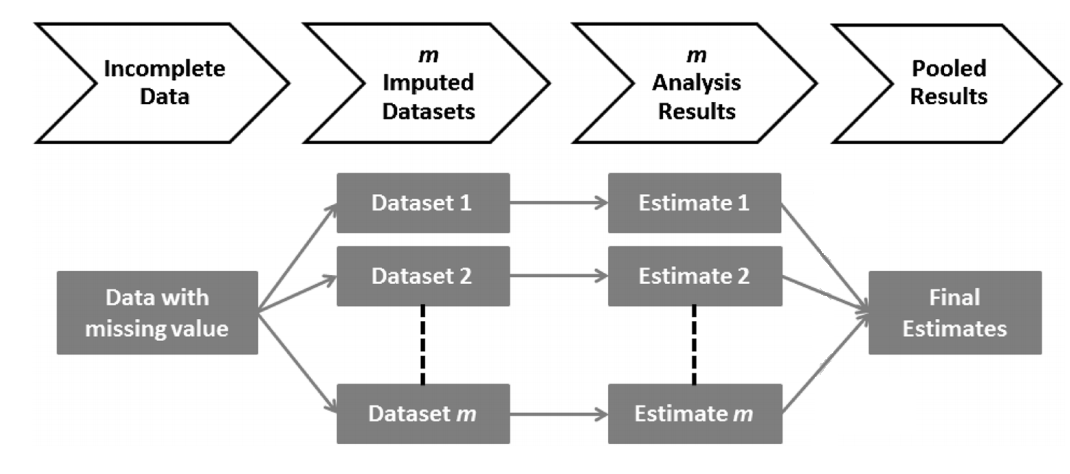
\includegraphics[width=\textwidth]{MultipleImputationPicture.PNG}
		\caption{An graphical layout of multiple imputation. At the start a dataset with missing values is present. Missing values are imputed $m$ times to create $m$ imputed datasets. The $m$ complete datasets are all analysed for $m$ different sets of estimates. These results are then pooled into one complete set of estimates.\cite{chevret2015multiple, rubin1976inference}}
		\label{fig:MultipleImputationLayout}
	\end{figure}
		
		
	\begin{itemize}
		
		\item \textit{Value imputation} \\
		The value imputation per dataset has different approaches available. One is similar to the previously discussed SI hot deck imputation. The quickest imputation would be to randomly choose a value from the distribution of the feature. After analysing all different datasets and combining them, it would seem as if the missing values were following the same distribution. Other techniques are similar to the multivariate regression imputation and the kNN imputation\cite{pedersen2017missing, white2011multiple}. The variance can be added manually. The variance is then averaged for all variances and in the end using a new averaged variance\cite{donders2006gentle}. Other mainly regression methods use different initial seeds as a way of creating a variance\cite{he2010multiple}.
		
		\item \textit{Additional datasets} \\
		The number of suggested datasets is different per study and usually differs between 3 and 10\cite{van2007multiple, pedersen2017missing, van1999multiple, van2006imputation, azur2011multiple, royston2004multiple}, however outliers of 15\cite{martin2018impact} and even 25\cite{raghunathan2001multivariate} are known. Other researchers even propose the number of datasets to be the same as the percentage of missing values\cite{white2011multiple}. The number of datasets is proportionally to the quality of the result and more datasets would indicate a better result. However generating and analysing more datasets also takes much more computation time, therefore a trade-off in computation time and quality should be considered.
		
		\item \textit{Analysis} \\
		The analysis of the dataset is project specific. Fro examples, if the outcome should be a linear equation between features and output, linear regression should be used to compute such an equation. Usually the outcome of such an analysis is more precise than it actually should be. By doing the same analysis multiple times with MI, a measure of uncertainty can be given to the outcome. This is done by combining the different outcomes together to one final outcome, by for example show standard deviations per regression coefficient\cite{donders2006gentle, van2006imputation}.
		
	\end{itemize}	

	% Advantages and disadvantages
	The main advantage of multiple imputation is the addition of uncertainty for imputation. In single imputation this uncertainty is unfairly low, which can create bias in results. Because of it being an extension on single imputation, it also inherits the advantages of being able to handle MAR values and possibly MNAR, and raises the number of samples to be used for analysis\cite{van2006imputation, pedersen2017missing}. The disadvantages mainly consist of taking up more computation time, due to multiplication of the analysis for the datasets. Therefore complex analysis techniques that take longer to compute may become unusable. Another aspect is the error given to missing value imputations. Not all analysis techniques perform well with errors which may create worse results even after combining the results\cite{pedersen2017missing}.
	
	% Implementations and MICE
	Several MI implementations are created and also added to mainly statistical analysis programs as SOLAS, SAS, SPSS, S-Plus and Stata\cite{horton2001multiple, allison2000multiple, royston2011multiple}. The most used implementation is multiple imputation for chained equations (MICE)\cite{azur2011multiple, royston2004multiple}, also known as sequential regression multiple implementation (SRMI)\cite{he2010multiple}. MICE stores the location of the missing values and iteratively replaces them with new values, according to a six step system\cite{azur2011multiple}. 
	
	\begin{enumerate}
		\item Replace all missing values with the mean of the corresponding feature.
		\item Choose a feature $f$ and remove the imputed values on all missing value locations.
		\item Create a model with all samples that do not have a missing value in $f$ to predict the value in $f$ by the other features.
		\item Impute the values in $f$ using the created model.
		\item Repeat steps 2 to 4 for all features that have missing values.
		\item Iteratively repeat steps 2 to 5 $s$ cycles for better more precise imputed values to create a final dataset.
	\end{enumerate}

	% Continuation MICE implementation
	The six steps create one dataset. The steps are $m$ times with different orders of choosing $f$ to create $m$ different datasets for analysis. The number of cycles used in the sixth step influences the precision of the outcome, as eventually the imputed missing values are expected to converge to one value. Usually about 10 cycles are done, as it is a good equilibrium between low computation time and high imputed value precision\cite{azur2011multiple, royston2004multiple}.
	
	%\subsection{Outlier Detection}
	%\label{subsec:OutlierDetection}
	
	\section{Methods}
	\label{sec:Methods}
	
	% Introduction
	To determine the quality of different missing value handling algorithms, two different approaches are used. The first approach focuses on the distributions of the different features and whether the algorithms create a bias in feature distributions. The second approach focuses on the evaluation quality and which missing value handling algorithm works best on predicting output.
	
	\subsection{Bias Evaluation}
	\label{subsec:BiasEvaluation}

	% Introduction
	After manipulating a dataset, the distributions of a feature can change significantly. This change in distribution can create a bias in the results and must be prevented as much as possible. To find out whether this bias is present, feature type specific values are compared between both the old and new feature values and those are compared using several statistical methods.
	
	% Statistical distribution measurement methods
	For future mentions of the two distributions that are compared the names 'old data' (before list deletion or value imputation) and 'new data' (after list deletion or value imputation) are used. The statistical methods that are used to find bias all are based on the same hypothesis H0: the old data and new data originate from the same distribution. This means the rejection hypothesis becomes H1: old and new data do not originate from the same distribution. Since features were nominal, ordinal or categorical, every feature type hypothesis is evaluated differently:
	
	\begin{itemize}
		\item \textit{Nominal features} \\
		For nominal features the mean and variance are main aspects to compare nominal distributions. To either accept the hypothesis, these two aspects are tested. The mean comparisons were done by using the known t-test\cite{heiberger2004statistical}. The equality of variance is tested by using a Levene's test with the Brown and Forsythe adaptation. This variance test was chosen due to not having any major assumptions on the distributions, for example the normality distribution\cite{brown1974robust}.
		\item \textit{Ordinal features} \\
		For ordinal features the mean cannot be used, as values are either not numeric or only give an indication with the numeric values. Because of that the median is used instead. The hypothesis is tested by checking whether this median is the same for both the old and new values. To have a better look at the distribution of the ordinal values, also a chi square test is done. This chi square test computes whether the distribution of ordinal values is the same for both the old and new values\cite{satorra2001scaled}.
		\item \textit{Categorical features} \\
		Categorical features do not have a mean or median, due to no ordering being present. Therefore the mode of the old and the new distribution is checked to be the same, to test the hypothesis H0 to be true. On top of that, the chi square test is here used, to find out whether the features from before and after the missing values algorithms can follow the same distribution\cite{satorra2001scaled}.
	\end{itemize}
	
	% Missing Value Handling Algorithms
	All features from the four datasets are tested whether any bias is present or not. The missing values are handled by seven different algorithms: CCA (Algorithm \ref{alg:CCA}), ACA (Algorithm \ref{alg:ACA}), Mean/Median/Mode imputation (Algorithm \ref{alg:MeanImputation}), Hot Deck imputation (Algorithm \ref{alg:HotDeckImputation}), kNN imputation (Algorithm \ref{alg:kNNImputation}), Regression imputation(Algorithm \ref{alg:RegressionImputation}) and at last MICE (Subsection \ref{subsec:MultipleImputation}). An overview of the datasets, evaluation tests and the missing value handling algorithms is provided (Table \ref{tab:BiasEvaluationTable}).
	
	\begin{table}[]
		\caption{The three different aspects of the bias evaluation. Four different datasets are used. Two tests are done per feature type, to test hypothesis H0 and seven missing value handling algorithms are implemented to be tested.}
		\label{tab:BiasEvaluationTable}
		\begin{tabular}{l|l|l}
			\textbf{Datasets}   & \begin{tabular}[c]{@{}l@{}}Heart Attack dataset\\ Hepatitis dataset\\ Cirrhosis dataset\\ Cervical cancer dataset\end{tabular}                                      & \begin{tabular}[c]{@{}l@{}}All datasets containing missing values \\ that are evaluated\end{tabular}                                                                                        \\ \hline
			\textbf{Test types} & \begin{tabular}[c]{@{}l@{}}Nominal features (t-test, levene's test)\\ Ordinal features  (median, chi-square)\\ Categorical features (mode, chi-square)\end{tabular} & \begin{tabular}[c]{@{}l@{}}Different types of features have different \\ tests for hypothesis H0: The old and \\ new distributions are the same\end{tabular}                                \\ \hline
			\textbf{Methods}    & \begin{tabular}[c]{@{}l@{}}CCA\\ WCA\\ Mean/Median/Mode imputation\\ Hot deck imputation\\ kNN imputation\\ Regression imputation\\ MICE\end{tabular}               & \begin{tabular}[c]{@{}l@{}}All methods to handle missing values:\\ - Two List Deletion algorithms\\ - Four Single Imputation algorithms\\ - One Multiple Imputation algorithms\end{tabular}
		\end{tabular}
	\end{table}
	
	% Tables
	The outcome of all the tests are shown in multiple tables. In those tables tests that show a rejection of H0 are highlighted. For the list deletion algorithms, additionally the type of missing values is evaluated by also testing the change in distribution in values without missing values. If a feature distribution changes for a feature without missing values after removing all missing values, a relation is present and the missing values are not MCAR. Aside from these tables plots of the relation between the percentage of missing values and probability of bias being present are made for every algorithm. This can indicate quality between the different algorithms with regards of the statistical hypothesis.

	\subsection{Quality Evaluation}
	\label{subsec:QualityEvaluation}
	
	\section{Results}
	\label{sec:Results}
	
	\subsection{Bias Evaluation Results}
	\label{subsec:BiasEvaluationResults}
	
	% Tables in appendix
	The outcome of the distribution tests for the heart attack dataset are visualised (Tables \ref{tab:LDHeartAttack} and \ref{tab:ImputationHeartAttack}), as well as the tables for the other datasets (Appendix \ref{app:DistributionTables}). The tables are split between list deletion (Table \ref{tab:LDHeartAttack}) and imputation (Table \ref{tab:ImputationHeartAttack}) results.
	
	\begin{table}[H]
		\caption{Testing for the heart attack data set whether the type of missing values can be represented by the remaining values. This is done by comparing distributions between the old and new data after CCA and WCA. For nominal values, two tests were used, an independent t-test for equality of mean and a Levene's test with the median in brackets to test equality of variance. For ordinal and categorical features the medians and modes where compared respectively as well as a chi squared test in brackets for equality of distribution. P-values lower than $p < 0.05$ are marked red for failure of representation, p-values higher than $p > 0.05$ are marked green for correctly being represented. If at least one feature is not represented after CCA, the missing values cannot be MCAR. If at least one feature is not represented after WCA, the pseudo-randomness cannot be corrected by only using weights for other values.}
		\label{tab:LDHeartAttack}
		\begin{tabular}{l|lll|lll|lll}
			\textbf{\begin{tabular}[c]{@{}l@{}}Feature \\ name\end{tabular}} & \textbf{\begin{tabular}[c]{@{}l@{}}still\\ alive\end{tabular}} & \textbf{age}                                                                             & \textbf{\begin{tabular}[c]{@{}l@{}}peri-\\ cardial\end{tabular}} & \textbf{\begin{tabular}[c]{@{}l@{}}frac-\\ tional\end{tabular}}                          & \textbf{epss}                                                                 & \textbf{lvdd}                                                                 & \textbf{\begin{tabular}[c]{@{}l@{}}wall\\ score\end{tabular}}                            & \textbf{\begin{tabular}[c]{@{}l@{}}wall\\ index\end{tabular}}                 & \textbf{\begin{tabular}[c]{@{}l@{}}alive\\ at 1\end{tabular}} \\ \hline
			\textbf{\begin{tabular}[c]{@{}l@{}}Value \\ type\end{tabular}}   & Cat                                                            & Nom                                                                                     & Cat                                                              & Nom                                                                                     & Nom                                                                          & Nom                                                                          & Nom                                                                                     & Nom                                                                          & Cat                                                           \\
			\textbf{Missing}   & 0\%                                                            & 3.85\%                                                                                   & 0\%                                                              & 5.38\%                                                                                   & 10.77\%                                                                       & 7.69\%                                                                        & 2.31\%                                                                                   & 0.77\%                                                                        & 43.85\%                                                       \\ \hline
			\textbf{\begin{tabular}[c]{@{}l@{}}p-values \\ CCA\end{tabular}} & \cellcolor[HTML]{009901}\begin{tabular}[c]{@{}l@{}}True\\ (0.96)\end{tabular}                        & \cellcolor[HTML]{9A0000}\begin{tabular}[c]{@{}l@{}}\textless{}0.01\\ (0.39)\end{tabular} & \cellcolor[HTML]{009901}\begin{tabular}[c]{@{}l@{}}True\\ (0.99)\end{tabular}                          & \cellcolor[HTML]{9A0000}\begin{tabular}[c]{@{}l@{}}\textless{}0.01\\ (0.83)\end{tabular} & \cellcolor[HTML]{009901}\begin{tabular}[c]{@{}l@{}}0.99\\ (0.74)\end{tabular} & \cellcolor[HTML]{009901}\begin{tabular}[c]{@{}l@{}}0.99\\ (0.94)\end{tabular} & \cellcolor[HTML]{9A0000}\begin{tabular}[c]{@{}l@{}}\textless{}0.01\\ (0.98)\end{tabular} & \cellcolor[HTML]{009901}\begin{tabular}[c]{@{}l@{}}0.09\\ (0.84)\end{tabular} & \cellcolor[HTML]{009901}\begin{tabular}[c]{@{}l@{}}True\\ (0.94)\end{tabular}                                  \\
			\textbf{\begin{tabular}[c]{@{}l@{}}p-values\\ WCA\end{tabular}}  & \cellcolor[HTML]{009901}\begin{tabular}[c]{@{}l@{}}True\\ (1.00)\end{tabular}                                  & \cellcolor[HTML]{009901}\begin{tabular}[c]{@{}l@{}}0.48\\ (0.82)\end{tabular}            & \cellcolor[HTML]{009901}\begin{tabular}[c]{@{}l@{}}True\\ (0.98)\end{tabular}                         & \cellcolor[HTML]{9A0000}\begin{tabular}[c]{@{}l@{}}\textless{}0.01\\ (0.45)\end{tabular} & \cellcolor[HTML]{009901}\begin{tabular}[c]{@{}l@{}}0.99\\ (0.39)\end{tabular} & \cellcolor[HTML]{009901}\begin{tabular}[c]{@{}l@{}}0.99\\ (0.28)\end{tabular} & \cellcolor[HTML]{9A0000}\begin{tabular}[c]{@{}l@{}}\textless{}0.01\\ (0.54)\end{tabular} & \cellcolor[HTML]{009901}\begin{tabular}[c]{@{}l@{}}0.99\\ (0.91)\end{tabular} & \cellcolor[HTML]{009901}\begin{tabular}[c]{@{}l@{}}True\\ (0.92)\end{tabular}                      
		\end{tabular}
	\end{table}
	
	% Observations in tables
	The tables show that in the heart attack, cirrhosis and cervical cancer datasets at least one feature shows a difference between the old and new data. Highlights are shown for changes in distribution for all values:
	
	\begin{itemize}
		\item \textbf{Heart attack:} \textit{age}, \textit{fractional} and \textit{wall score} all have $p < 0.01$ for having the same mean before and after CCA. This indicates that the missing value type of at least one feature is MAR and for all three possibly even MNAR. WCA does help in creating a representative distribution for the feature \textit{age}, however \textit{fractional} and \textit{wall score} still are differently distributed. Other approaches to handle missing values are most likely more effective
		\item \textbf{Hepatitis:} For no feature a reason to reject the distributions before and after deleting samples with missing values is present. The feature that is least likely to have the same distribution is \textit{bilirubin} with having a $p = 0.14$ for the same mean and $p = 0.23$ for the same variance. We therefore cannot say that the missing values are MCAR and using only CCA to handle missing values is certainly possible. WCA has worse results for several features and show that WCA might not be the best way to improve the sample size for this dataset.
		\item \textbf{Cirrhosis:} \textit{case number}, \textit{status}, \textit{day}, \textit{albumin} and \textit{SGOT} all have $p < 0.05$ if nominal for having the same mean and \textit{False} if ordinal or categorical for having the same median or mode, respectively. These five features do not have missing values. This means that the bias in the distribution is caused by list deletion due to another feature's missing values. Therefore it can be concluded that least for one feature the missing values are at least MAR. WCA helps fixing the distributions for \textit{case number} and \textit{SGOT}, but also creates additional bias in \textit{presence of ascites}, \textit{presence of hepatocytes} and \textit{presence of edema} and therefore is not a suitable approach to remove possible bias. 
		\item \textbf{Cervical cancer:} \textit{STDs}, \textit{\#STDs}, \textit{condylomatosis}, \textit{vulvoperineal condlymatosis} and \textit{STDs \#diagnosis} all have $p < 0.05$ if nominal for having the same mean and \textit{False} if categorical for having the same mode. All but \textit{STDs \#diagnosis} also have a $p < 0.05$ for having the same variance if nominal or the same chi square distribution if categorical, which further strengthens hypothesis H1 of the distributions being different. This indicates that the missing values of at least one feature is MCAR.
	\end{itemize}

	\begin{table}[H]
		\caption{A table showing the number of samples that remained after performing CCA.}
		\label{tab:CCARemainingSamples}
		\begin{tabular}{l|l|l}
			\textbf{Dataset}      & \textbf{Total samples} & \textbf{\begin{tabular}[c]{@{}l@{}}Number of samples \\ after CCA\end{tabular}} \\ \hline
			\textbf{Heart Attack} & 108                    & 61                                                                                \\
			\textbf{Hepatitis}    & 155                    & 80                                                                                \\ \hline
			Cirrhosis             & 1945                   & 1113                                                                              \\
			Cervical Cancer       & 585                    & 59                                                                               
		\end{tabular}
	\end{table}

	The heart attack, cirrhosis and cervical cancer datasets all indicate possible bias after deleting samples with missing values. On top of that, after removing all samples with missing values not many samples are left for any of the datasets (Table \ref{tab:CCARemainingSamples}). The hepatitis dataset loses almost 50\% of its samples after CCA and the cervical cancer dataset drops down to only 10\% of its original values. All four datasets would therefore potentially benefit from an imputation approach.
	
	\begin{table}[]
		\caption{Testing for the heart attack data set if certain types of imputation create a vastly different distribution for features with missing values. The imputation values are generated with mean imputation, hot deck imputation, k-Nearest Neighbour imputation ($k = 3$), regression imputation and MICE (number of cycles is $s = 5$). For nominal values, two tests were used, an independent t-test for equality of mean and a Levene's test with the median in brackets to test equality of variance. For ordinal and categorical features the medians and modes where checked respectively to be similar as well as a chi squared test in brackets fro equality of distribution. P-values lower than $p < 0.05$ are marked red for failure of representation, p-values close to $p > 0.05$ are marked green for correctly being represented.}
		\label{tab:ImputationHeartAttack}
		\begin{tabular}{l|ll|lll|ll}
			\textbf{\begin{tabular}[c]{@{}l@{}}Feature \\ name\end{tabular}}         & \textbf{age}                                                                  & \textbf{\begin{tabular}[c]{@{}l@{}}frac-\\ tional\end{tabular}}               & \textbf{epss}                                                                 & \textbf{lvdd}                                                                 & \textbf{\begin{tabular}[c]{@{}l@{}}wall\\ score\end{tabular}}                 & \textbf{\begin{tabular}[c]{@{}l@{}}wall\\ index\end{tabular}}                 & \textbf{\begin{tabular}[c]{@{}l@{}}alive\\ at 1\end{tabular}} \\ \hline
			\textbf{\begin{tabular}[c]{@{}l@{}}Value \\ type\end{tabular}}           & Nom                                                                          & Nom                                                                          & Nom                                                                          & Nom                                                                          & Nom                                                                          & Nom                                                                          & Cat                                                           \\
			\textbf{Missing}          & 3.85\%                                                                        & 5.38\%                                                                        & 10.77\%                                                                       & 7.69\%                                                                        & 2.31\%                                                                        & 0.77\%                                                                        & 43.85\%                                                       \\ \hline
			\textbf{\begin{tabular}[c]{@{}l@{}}Mean\\ Imputation\end{tabular}}       & \cellcolor[HTML]{009901}\begin{tabular}[c]{@{}l@{}}1.00\\ (0.76)\end{tabular} & \cellcolor[HTML]{009901}\begin{tabular}[c]{@{}l@{}}0.99\\ (0.60)\end{tabular} & \cellcolor[HTML]{009901}\begin{tabular}[c]{@{}l@{}}0.99\\ (0.39)\end{tabular} & \cellcolor[HTML]{009901}\begin{tabular}[c]{@{}l@{}}1.00\\ (0.48)\end{tabular} & \cellcolor[HTML]{009901}\begin{tabular}[c]{@{}l@{}}1.00\\ (0.88)\end{tabular} & \cellcolor[HTML]{009901}\begin{tabular}[c]{@{}l@{}}1.00\\ (0.98)\end{tabular} & \cellcolor[HTML]{009901}\begin{tabular}[c]{@{}l@{}}True\\ (0.77)\end{tabular}                      \\
			\textbf{\begin{tabular}[c]{@{}l@{}}Hot Deck\\ Imputation\end{tabular}}   & \cellcolor[HTML]{009901}\begin{tabular}[c]{@{}l@{}}0.97\\ (0.98)\end{tabular} & \cellcolor[HTML]{009901}\begin{tabular}[c]{@{}l@{}}0.88\\ (0.88)\end{tabular} & \cellcolor[HTML]{009901}\begin{tabular}[c]{@{}l@{}}0.94\\ (0.98)\end{tabular} & \cellcolor[HTML]{009901}\begin{tabular}[c]{@{}l@{}}0.82\\ (0.91)\end{tabular} & \cellcolor[HTML]{009901}\begin{tabular}[c]{@{}l@{}}0.94\\ (0.86)\end{tabular} & \cellcolor[HTML]{009901}\begin{tabular}[c]{@{}l@{}}0.96\\ (0.96)\end{tabular} & \cellcolor[HTML]{009901}\begin{tabular}[c]{@{}l@{}}True\\ ( 0.96)\end{tabular}                      \\ \hline
			\textbf{\begin{tabular}[c]{@{}l@{}}kNN\\ Imputation\end{tabular}}        & \cellcolor[HTML]{009901}\begin{tabular}[c]{@{}l@{}}0.86\\ (0.99)\end{tabular} & \cellcolor[HTML]{009901}\begin{tabular}[c]{@{}l@{}}0.81\\ (0.88)\end{tabular} & \cellcolor[HTML]{009901}\begin{tabular}[c]{@{}l@{}}0.69\\ (0.62)\end{tabular} & \cellcolor[HTML]{009901}\begin{tabular}[c]{@{}l@{}}0.94\\ (0.68)\end{tabular} & \cellcolor[HTML]{009901}\begin{tabular}[c]{@{}l@{}}0.96\\ (0.97)\end{tabular} & \cellcolor[HTML]{009901}\begin{tabular}[c]{@{}l@{}}0.96\\ (0.98)\end{tabular} & \cellcolor[HTML]{009901}\begin{tabular}[c]{@{}l@{}}True\\ (0.91)\end{tabular}                       \\
			\textbf{\begin{tabular}[c]{@{}l@{}}Regression\\ Imputation\end{tabular}} & \cellcolor[HTML]{009901}\begin{tabular}[c]{@{}l@{}}0.84\\ (1.00)\end{tabular} & \cellcolor[HTML]{009901}\begin{tabular}[c]{@{}l@{}}0.71\\ (0.95)\end{tabular} & \cellcolor[HTML]{009901}\begin{tabular}[c]{@{}l@{}}0.34\\ (0.57)\end{tabular} & \cellcolor[HTML]{009901}\begin{tabular}[c]{@{}l@{}}0.91\\ (0.76)\end{tabular} & \cellcolor[HTML]{009901}\begin{tabular}[c]{@{}l@{}}0.88\\ (1.00)\end{tabular} & \cellcolor[HTML]{009901}\begin{tabular}[c]{@{}l@{}}0.93\\ (0.98)\end{tabular} & \cellcolor[HTML]{009901}\begin{tabular}[c]{@{}l@{}}True\\ (0.92)\end{tabular}                       \\ \hline
			\textbf{\begin{tabular}[c]{@{}l@{}}MICE\\ (5 cycles)\end{tabular}}       & \cellcolor[HTML]{009901}\begin{tabular}[c]{@{}l@{}}0.97\\ (0.81)\end{tabular} & \cellcolor[HTML]{009901}\begin{tabular}[c]{@{}l@{}}0.94\\ (0.80)\end{tabular} & \cellcolor[HTML]{009901}\begin{tabular}[c]{@{}l@{}}0.98\\ (0.90)\end{tabular} & \cellcolor[HTML]{009901}\begin{tabular}[c]{@{}l@{}}0.80\\ (0.84)\end{tabular} & \cellcolor[HTML]{009901}\begin{tabular}[c]{@{}l@{}}0.98\\ (0.98)\end{tabular} & \cellcolor[HTML]{009901}\begin{tabular}[c]{@{}l@{}}0.96\\ (0.97)\end{tabular} & \cellcolor[HTML]{009901}\begin{tabular}[c]{@{}l@{}}True\\ (0.93)\end{tabular}                      
		\end{tabular}
	\end{table}

	% Imputation methods
	Most imputation methods show an improvement in results The heart attack dataset has no bias in distributions after any of the five tested imputation methods, the hepatitis dataset only has bias when using mean imputation or MICE, the cirrhosis dataset only shows bias when using mean imputation and at last in the cervical cancer dataset all but the two features with 91.75\% missing values contain no bias between distributions. On top of that, the only features that had bias in the newly created distributions are features with more than 40\% missing values, indicating that imputation methods have more problems when a higher missing/not missing ratio is present. this gives an indication that removal of features with missing values higher than 40\% would greatly help the usefulness of a dataset.
	
	% Plotting imputation methods
	A scatter plot with fitted linear curves is made to show a relation between the probability of the old and new mean (Figure \ref{fig:PMeanFits}) and variance (Figure \ref{fig:PVarianceFits}) originating from the same distribution and the percentage of values missing. For these fits, features with more than 15\% of missing values were removed due to not being properly represented by nominal features in the four datasets. The fitted lines by no means show a perfect fit, but they do show the trend of the missing value handling algorithms. 
	
	\begin{figure}[H]
		\centering
		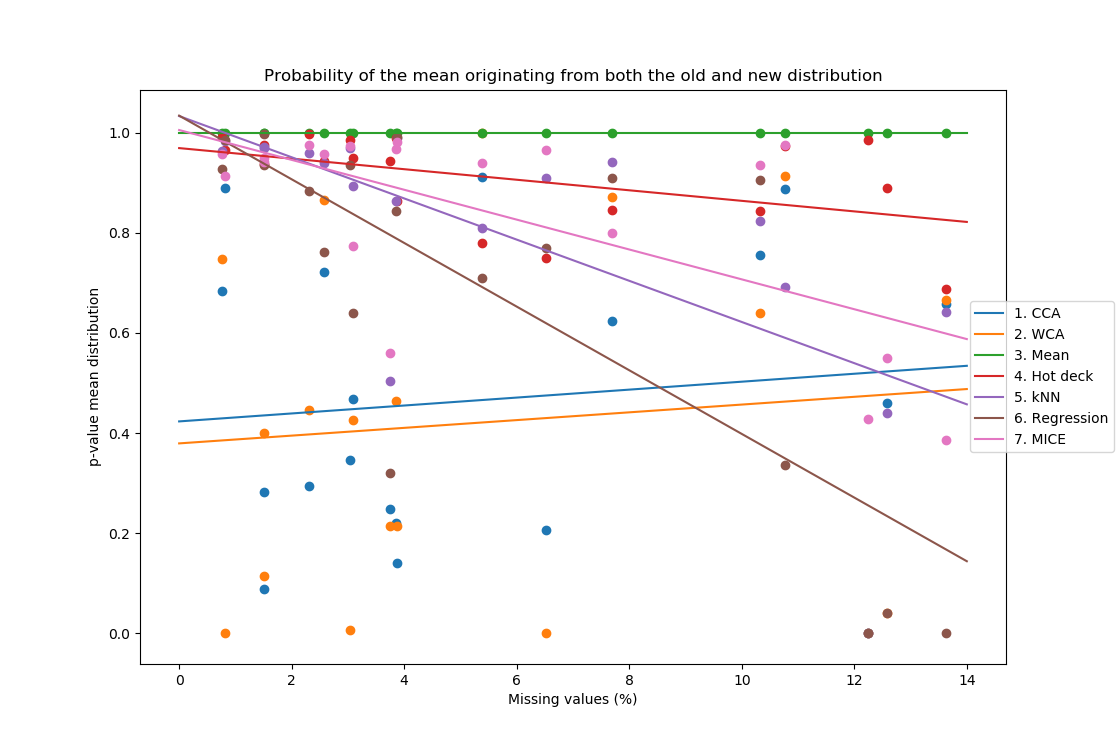
\includegraphics[width=\textwidth]{P_mean.PNG}
		\caption{The probability of the mean of the old and new distribution originating from the same distribution. On the x-axis the percentage of missing values is given for a feature and on the y-axis the p-value of the probability. For every missing value algorithm also a linear fit is made to show the trend of the scatter plot.}
		\label{fig:PMeanFits}
	\end{figure}
	
	\begin{figure}[H]
		\centering
		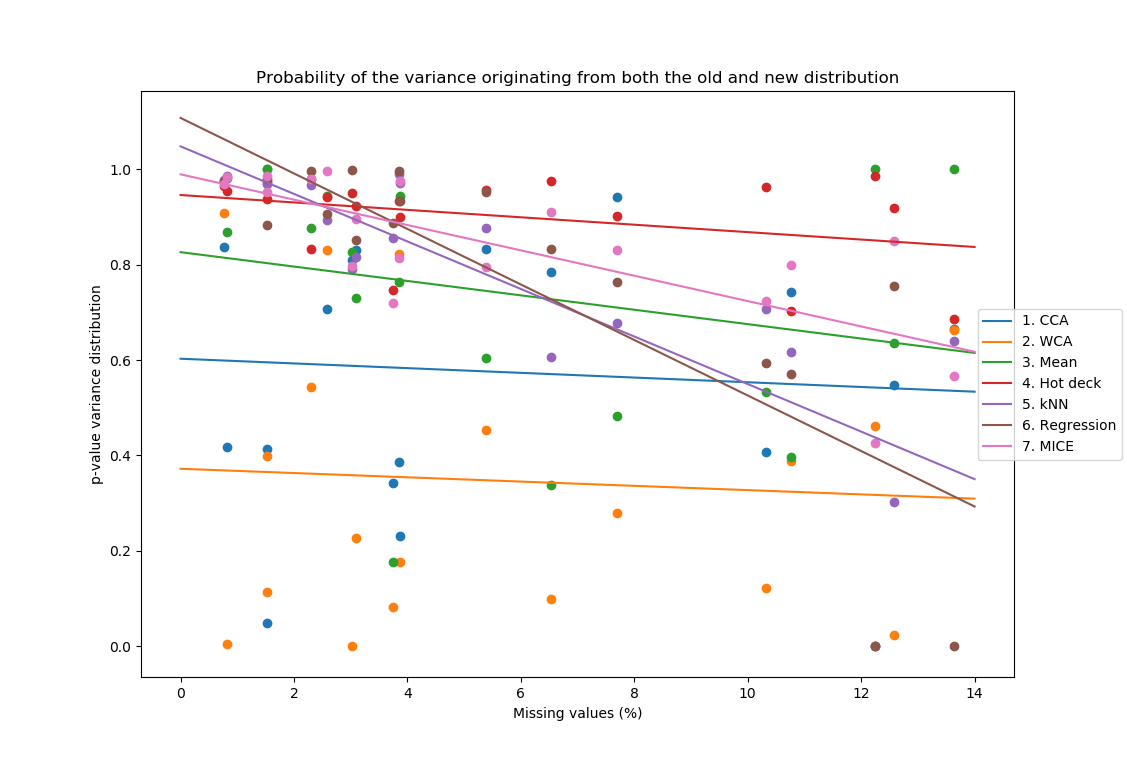
\includegraphics[width=\textwidth]{P_variance.PNG}
		\caption{The probability of the variance of the old and new distribution originating from the same distribution. On the x-axis the percentage of missing values is given for a feature and on the y-axis the p-value of the probability. For every missing value algorithm also a linear fit is made to show the trend of the scatter plot.}
		\label{fig:PVarianceFits}
	\end{figure}
	
	% List deletion
	List Deletion algorithms seem to be better at creating a representative distribution when more missing values are present. This is explainable for these datasets as all of them have a at least one feature with more than 40\%. Most samples are removed because of this feature also removing significant portions of other features. This results in features having more missing values will leave them with a higher percentage of their original values, therefore being closer to the original values.
	
	% Imputation
	The imputation algorithm seem to show big differences between the results. Hot deck imputation seems to create the best representative distribution, being the best when comparing mean and variance for the old and new distribution. Mean Imputation obviously shows a perfect fit for comparing means, however for variance imputation it is worse than both hot deck and MICE. It does show a less steep slope than MICE, so for more than 15\% missing values it may show a better result. kNN imputation, regression imputation and MICE all show good results at low percentages, however these results worsen significantly more when more missing values are present. Of these three, MICE shows the best distribution results, followed by kNN imputation and at last regression imputation.
	
	% Explanation quality mean and hot deck
	The high quality for both mean and hot deck imputation can be explained by the evaluation methods. A mean comparison for mean imputation is obviously perfect, and the variance will always become smaller when more means are imputed. Hot deck imputation adds values according to the distribution of the features. This distribution follows the mean and variance of the original values and therefore the mean and variance will always be close to the original distribution. When looking at other aspects, for example the ability to predict the output with the dataset, hot deck imputation and mean imputation should show worse results as distribution specific estimations were imputed, instead of sample specific.
	
	\section{Conclusions}
	\label{sec:Conclusions}
	
	\section{Discussion}
	\label{sec:Discussion}
	
	\bibliography{../References/Citings} 
	\bibliographystyle{ieeetr}
	
	\appendix
	
	\section{Feature Distribution Tables}
	\label{app:DistributionTables}
	
	% Introduction
	The distribution tables for the hepatitis (Tables \ref{tab:LDHepatitis} and \ref{tab:ImputationHepatitis}), cirrhosis (Tables \ref{tab:LDCirrhosis} and \ref{tab:ImputationCirrhosis}) and cervical cancer (Table \ref{tab:LDCervical}) datasets. For the hepatitis and cirrhosis datasets the tables are split in list deletion (Tables \ref{tab:LDHepatitis} and \ref{tab:LDCirrhosis}) and imputation (Tables \ref{tab:ImputationHepatitis} and \ref{tab:ImputationCirrhosis}). For the cervical cancer dataset both tables were combined due to not being any significant difference between the imputation technique outcomes. 
	
	\begin{sidewaystable}[]
		\caption{Testing for the hepatitis data set whether the type of missing values can be represented by the remaining values. This is done by comparing distributions between all sample values and remaining sample values after CCA and WCA. For nominal values, two tests were used, an independent t-test for equality of mean and a Levene's test with the median in brackets to test equality of variance. For ordinal and categorical features the medians and modes where checked respectively to be similar as well as a chi squared test in brackets fro equality of distribution. P-values lower than $p < 0.05$ are marked red for failure of representation, p-values higher than $p > 0.05$ are marked green for correctly being represented. If at least one feature is not represented after CCA, the missing values cannot be MCAR. If at least one feature is not represented after WCA, the pseudo-randomness cannot be corrected by only using weights for other values.}
		\label{tab:LDHepatitis}
		\begin{tabular}{l|lll|lll|llll}
			\textbf{\begin{tabular}[c]{@{}l@{}}Feature \\ name\end{tabular}}  & \textbf{age}                                                                  & \textbf{sex}                                                 & \textbf{steroid}                                             & \textbf{\begin{tabular}[c]{@{}l@{}}anti-\\ virals\end{tabular}}               & \textbf{\begin{tabular}[c]{@{}l@{}}fat-\\ igue\end{tabular}}                                                               & \textbf{\begin{tabular}[c]{@{}l@{}}mal-\\ aise\end{tabular}}                                                              & \textbf{\begin{tabular}[c]{@{}l@{}}ano-\\ rexia\end{tabular}}                 & \textbf{\begin{tabular}[c]{@{}l@{}}liver\\ big\end{tabular}}                  & \textbf{\begin{tabular}[c]{@{}l@{}}liver\\ firm\end{tabular}} & \textbf{\begin{tabular}[c]{@{}l@{}}spleen\\ palpable\end{tabular}} \\ \hline
			\textbf{\begin{tabular}[c]{@{}l@{}}Value \\ type\end{tabular}}    & Nom                                                                          & Cat                                                          & Cat                                                          & Cat                                                                           & Cat                                                                            & Cat                                                                           & Cat                                                                           & Cat                                                                           & Cat                                                           & Cat                                                                \\
			\textbf{Missing}                                                  & 0\%                                                                           & 0\%                                                          & 0.65\%                                                       & 0\%                                                                           & 0.65\%                                                                         & 0.65\%                                                                        & 0.65\%                                                                        & 6.45\%                                                                        & 7.10\%                                                        & 3.23\%                                                             \\ \hline
			\textbf{\begin{tabular}[c]{@{}l@{}}p-values \\ CCA\end{tabular}}  & \cellcolor[HTML]{009901}\begin{tabular}[c]{@{}l@{}}0.74\\ (0.30)\end{tabular} & \cellcolor[HTML]{009901}\begin{tabular}[c]{@{}l@{}}True\\ (0.91)\end{tabular}                      & \cellcolor[HTML]{009901}\begin{tabular}[c]{@{}l@{}}True\\ (0.97)\end{tabular}                      & \cellcolor[HTML]{009901}\begin{tabular}[c]{@{}l@{}}True\\ (0.77)\end{tabular}                                      & \cellcolor[HTML]{009901}\begin{tabular}[c]{@{}l@{}}True\\ (1.00)\end{tabular}                                        & \cellcolor[HTML]{009901}\begin{tabular}[c]{@{}l@{}}True\\ (0.99)\end{tabular}                                       & \cellcolor[HTML]{009901}\begin{tabular}[c]{@{}l@{}}True\\ (0.89)\end{tabular}                                      & \cellcolor[HTML]{009901}\begin{tabular}[c]{@{}l@{}}True\\ (0.98)\end{tabular}                                       & \cellcolor[HTML]{009901}\begin{tabular}[c]{@{}l@{}}True\\ (0.91)\end{tabular}                      & \cellcolor[HTML]{009901}\begin{tabular}[c]{@{}l@{}}True\\ (0.98)\end{tabular}                           \\
			\textbf{\begin{tabular}[c]{@{}l@{}}p-values\\ WCA\end{tabular}}   & \cellcolor[HTML]{009901}\begin{tabular}[c]{@{}l@{}}0.63\\ (0.24)\end{tabular} & \cellcolor[HTML]{009901}\begin{tabular}[c]{@{}l@{}}True\\ (1.00)\end{tabular}                                 & \cellcolor[HTML]{9A0000}\begin{tabular}[c]{@{}l@{}}False\\ (0.98)\end{tabular}                                & \cellcolor[HTML]{009901}\begin{tabular}[c]{@{}l@{}}True\\ (1.00)\end{tabular}                                                & \cellcolor[HTML]{009901}\begin{tabular}[c]{@{}l@{}}True\\ (1.00)\end{tabular}                                                   & \cellcolor[HTML]{009901}\begin{tabular}[c]{@{}l@{}}True\\ (0.96)\end{tabular}                                                  & \cellcolor[HTML]{009901}\begin{tabular}[c]{@{}l@{}}True\\ (0.92)\end{tabular}                                                  & \cellcolor[HTML]{009901}\begin{tabular}[c]{@{}l@{}}True\\ (0.96)\end{tabular}                                                 & \cellcolor[HTML]{009901}\begin{tabular}[c]{@{}l@{}}True\\ (0.94)\end{tabular}                                 & \cellcolor[HTML]{009901}\begin{tabular}[c]{@{}l@{}}True\\ (0.96)\end{tabular}                                      \\ \hline
			\textbf{\begin{tabular}[c]{@{}l@{}}Feature\\ name\end{tabular}}   & \textbf{\begin{tabular}[c]{@{}l@{}}spi-\\ders\end{tabular}} & 
			\textbf{\begin{tabular}[c]{@{}l@{}}as-\\ cites\end{tabular}} & \textbf{\begin{tabular}[c]{@{}l@{}}var-\\ ices\end{tabular}} & \textbf{\begin{tabular}[c]{@{}l@{}}bili-\\ rubin\end{tabular}}                & \textbf{\begin{tabular}[c]{@{}l@{}}alk \\ phos-\\ phate\end{tabular}}          & \textbf{sgot}                                                                 & \textbf{\begin{tabular}[c]{@{}l@{}}albu-\\ min\end{tabular}}                  & \textbf{\begin{tabular}[c]{@{}l@{}}pro-\\ time\end{tabular}}                  & \textbf{\begin{tabular}[c]{@{}l@{}}hist-\\ ology\end{tabular}}                     & \textbf{}                                                          \\ \cline{1-10}
			\textbf{\begin{tabular}[c]{@{}l@{}}Value \\ type\end{tabular}}    & Cat                                                                           & Cat                                                          & Cat                                                          & Nom                                                                          & Nom                                                                           & Nom                                                                          & Nom                                                                          & Nom                                                                          & Cat                                                                                &                                                                    \\
			\textbf{Missing} & 3.23\%                                                                        & 3.23\%                                                       & 3.23\%                                                       & 3.87\%                                                                        & 18.71\%                                                                        & 2.58\%                                                                        & 10.32\%                                                                       & 43.23\%                                                                       & 0\%                                                                                &                                                                    \\ \cline{1-10}
			\textbf{\begin{tabular}[c]{@{}l@{}}p-values\\ CCA\end{tabular}}   & \cellcolor[HTML]{009901}\begin{tabular}[c]{@{}l@{}}True\\ (0.95)\end{tabular}                                       & \cellcolor[HTML]{009901}\begin{tabular}[c]{@{}l@{}}True\\ (0.96)\end{tabular}                      & \cellcolor[HTML]{009901}\begin{tabular}[c]{@{}l@{}}True\\ (0,99)\end{tabular}                     & \cellcolor[HTML]{009901}\begin{tabular}[c]{@{}l@{}}0.14\\ (0.23)\end{tabular} & \cellcolor[HTML]{009901}\begin{tabular}[c]{@{}l@{}}0.75\\ (0.71)\end{tabular}  & \cellcolor[HTML]{009901}\begin{tabular}[c]{@{}l@{}}0.72\\ (0.71)\end{tabular} & \cellcolor[HTML]{009901}\begin{tabular}[c]{@{}l@{}}0.76\\ (0.41)\end{tabular} & \cellcolor[HTML]{009901}\begin{tabular}[c]{@{}l@{}}0.85\\ (0.83)\end{tabular} & \cellcolor[HTML]{009901}\begin{tabular}[c]{@{}l@{}}True\\ (0.94)\end{tabular}                                            &                                                                    \\
			\textbf{\begin{tabular}[c]{@{}l@{}}p-values\\ WCA\end{tabular}}   & \cellcolor[HTML]{009901}\begin{tabular}[c]{@{}l@{}}True\\ (0.99)\end{tabular}                                                 & \cellcolor[HTML]{009901}\begin{tabular}[c]{@{}l@{}}True\\ (0.99)\end{tabular}                                & \cellcolor[HTML]{009901}\begin{tabular}[c]{@{}l@{}}True\\ (0.99)\end{tabular}                                & \cellcolor[HTML]{009901}\begin{tabular}[c]{@{}l@{}}0.21\\ (0.18)\end{tabular} & \cellcolor[HTML]{009901}\begin{tabular}[c]{@{}l@{}}0.84\\ (0.60)\end{tabular} & \cellcolor[HTML]{009901}\begin{tabular}[c]{@{}l@{}}0.87\\ (0.83)\end{tabular} & \cellcolor[HTML]{009901}\begin{tabular}[c]{@{}l@{}}0.64\\ (0.12)\end{tabular} & \cellcolor[HTML]{009901}\begin{tabular}[c]{@{}l@{}}0.66\\ (0.29)\end{tabular} & \cellcolor[HTML]{009901}\begin{tabular}[c]{@{}l@{}}True\\ (0.95)\end{tabular}                                                       &                                                                   
		\end{tabular}
	\end{sidewaystable}
	
	\begin{sidewaystable}[]
		\caption{Testing for the hepatitis data set if certain types of imputation create a vastly different distribution for features with missing values. The imputation values are generated with mean imputation, hot deck imputation, k-Nearest Neighbour imputation ($k = 3$), regression imputation and MICE (number of cycles is $s = 5$). For nominal values, two tests were used, an independent t-test for equality of mean and a Levene's test with the median in brackets to test equality of variance. For ordinal and categorical features the medians and modes where checked respectively to be similar as well as a chi squared test in brackets fro equality of distribution. P-values lower than $p < 0.05$ are marked red for failure of representation, p-values close to $p > 0.05$ are marked green for correctly being represented.}
		\label{tab:ImputationHepatitis}
		\begin{tabular}{l|lll|lll|lll|lll|lll}
			\textbf{\begin{tabular}[c]{@{}l@{}}Feature \\ name\end{tabular}}         & \textbf{\begin{tabular}[c]{@{}l@{}}ste-\\ roid\end{tabular}} & \textbf{\begin{tabular}[c]{@{}l@{}}fat-\\ igue\end{tabular}} & \textbf{\begin{tabular}[c]{@{}l@{}}mal-\\ aise\end{tabular}} & \textbf{\begin{tabular}[c]{@{}l@{}}ano-\\ rexia\end{tabular}} & \textbf{\begin{tabular}[c]{@{}l@{}}liver\\ big\end{tabular}} & \textbf{\begin{tabular}[c]{@{}l@{}}liver\\ firm\end{tabular}} & \textbf{\begin{tabular}[c]{@{}l@{}}spleen\\ palpable\end{tabular}} & \textbf{\begin{tabular}[c]{@{}l@{}}spi-\\ ders\end{tabular}} & \textbf{\begin{tabular}[c]{@{}l@{}}as-\\ cites\end{tabular}} & \textbf{\begin{tabular}[c]{@{}l@{}}var-\\ ices\end{tabular}} & \textbf{\begin{tabular}[c]{@{}l@{}}bili-\\ rubin\end{tabular}}                & \textbf{\begin{tabular}[c]{@{}l@{}}alk\\ phos-\\ phate\end{tabular}}          & \textbf{sgot}                                                                 & \textbf{\begin{tabular}[c]{@{}l@{}}albu-\\ min\end{tabular}}                  & \textbf{\begin{tabular}[c]{@{}l@{}}pro-\\ time\end{tabular}}                             \\ \hline
			\textbf{\begin{tabular}[c]{@{}l@{}}Value \\ type\end{tabular}}           & Cat                                                          & Cat                                                          & Cat                                                          & Cat                                                           & Cat                                                          & Cat                                                           & Cat                                                                & Cat                                                          & Cat                                                          & Cat                                                          & Nom                                                                          & Nom                                                                          & Nom                                                                          & Nom                                                                          & Nom                                                                                     \\
			\textbf{Missing}         & 0.65\%                                                       & 0.65\%                                                       & 0.65\%                                                       & 0.65\%                                                        & 6.45\%                                                       & 7.10\%                                                        & 3.23\%                                                             & 3.23\%                                                       & 3.23\%                                                       & 3.23\%                                                       & 3.87\%                                                                        & 18.71\%                                                                       & 2.58\%                                                                        & 10.32\%                                                                       & 43.23\%                                                                                  \\ \hline
			\textbf{\begin{tabular}[c]{@{}l@{}}Mean\\ Imputation\end{tabular}}       & \cellcolor[HTML]{009901}\begin{tabular}[c]{@{}l@{}}True\\ (0.99)\end{tabular}                                 & \cellcolor[HTML]{009901}\begin{tabular}[c]{@{}l@{}}True\\ (1.00)\end{tabular}                                & \cellcolor[HTML]{009901}\begin{tabular}[c]{@{}l@{}}True\\ (0.96)\end{tabular}                                 & \cellcolor[HTML]{009901}\begin{tabular}[c]{@{}l@{}}True\\ (0.92)\end{tabular}                                  & \cellcolor[HTML]{009901}\begin{tabular}[c]{@{}l@{}}True\\ (0.96)\end{tabular}                                 & \cellcolor[HTML]{009901}\begin{tabular}[c]{@{}l@{}}True\\ (0.94)\end{tabular}                                  & \cellcolor[HTML]{009901}\begin{tabular}[c]{@{}l@{}}True\\ (0.98)\end{tabular}                                       & \cellcolor[HTML]{009901}\begin{tabular}[c]{@{}l@{}}True\\ (0.99)\end{tabular}                                 & \cellcolor[HTML]{009901}\begin{tabular}[c]{@{}l@{}}True\\ (0.99)\end{tabular}                                 & \cellcolor[HTML]{009901}\begin{tabular}[c]{@{}l@{}}True\\ (0.94)\end{tabular}                                 & \cellcolor[HTML]{009901}\begin{tabular}[c]{@{}l@{}}0.66\\ (0.94)\end{tabular} & \cellcolor[HTML]{009901}\begin{tabular}[c]{@{}l@{}}1.00\\ (0.33)\end{tabular} & \cellcolor[HTML]{009901}\begin{tabular}[c]{@{}l@{}}1.00\\ (0.94)\end{tabular} & \cellcolor[HTML]{009901}\begin{tabular}[c]{@{}l@{}}1.00\\ (0.53)\end{tabular} & \cellcolor[HTML]{9A0000}\begin{tabular}[c]{@{}l@{}}1.00\\ (\textless{}0.01)\end{tabular} \\
			\textbf{\begin{tabular}[c]{@{}l@{}}Hot Deck\\ Imputation\end{tabular}}   & \cellcolor[HTML]{009901}\begin{tabular}[c]{@{}l@{}}True\\ (0.99)\end{tabular}                                 & \cellcolor[HTML]{009901}\begin{tabular}[c]{@{}l@{}}True\\ (0.99)\end{tabular}                                & \cellcolor[HTML]{009901}\begin{tabular}[c]{@{}l@{}}True\\ (1.00)\end{tabular}                                 & \cellcolor[HTML]{009901}\begin{tabular}[c]{@{}l@{}}True\\ (0.99)\end{tabular}                                  & \cellcolor[HTML]{009901}\begin{tabular}[c]{@{}l@{}}True\\ (0.98)\end{tabular}                                 & \cellcolor[HTML]{009901}\begin{tabular}[c]{@{}l@{}}True\\ (0.97)\end{tabular}                                  & \cellcolor[HTML]{009901}\begin{tabular}[c]{@{}l@{}}True\\ (0.97)\end{tabular}                                       & \cellcolor[HTML]{009901}\begin{tabular}[c]{@{}l@{}}True\\ (0.99)\end{tabular}                                 & \cellcolor[HTML]{009901}\begin{tabular}[c]{@{}l@{}}True\\ (0.99)\end{tabular}                                 & \cellcolor[HTML]{009901}\begin{tabular}[c]{@{}l@{}}True\\ (0.99)\end{tabular}                                 & \cellcolor[HTML]{009901}\begin{tabular}[c]{@{}l@{}}0.94\\ (0.91)\end{tabular} & \cellcolor[HTML]{009901}\begin{tabular}[c]{@{}l@{}}0.77\\ (0.73)\end{tabular} & \cellcolor[HTML]{009901}\begin{tabular}[c]{@{}l@{}}0.98\\ (1.00)\end{tabular} & \cellcolor[HTML]{009901}\begin{tabular}[c]{@{}l@{}}0.98\\ (0.91)\end{tabular} & \cellcolor[HTML]{009901}\begin{tabular}[c]{@{}l@{}}0.84\\ (0.79)\end{tabular}            \\ \hline
			\textbf{\begin{tabular}[c]{@{}l@{}}kNN\\ Imputation\end{tabular}}        & \cellcolor[HTML]{009901}\begin{tabular}[c]{@{}l@{}}True\\ (0.99)\end{tabular}                                 & \cellcolor[HTML]{009901}\begin{tabular}[c]{@{}l@{}}True\\ (1.00)\end{tabular}                                 & \cellcolor[HTML]{009901}\begin{tabular}[c]{@{}l@{}}True\\ (0.99)\end{tabular}                                 & \cellcolor[HTML]{009901}\begin{tabular}[c]{@{}l@{}}True\\ (1.00)\end{tabular}                                  & \cellcolor[HTML]{009901}\begin{tabular}[c]{@{}l@{}}True\\ (0.98)\end{tabular}                                 & \cellcolor[HTML]{009901}\begin{tabular}[c]{@{}l@{}}True\\ (0.97)\end{tabular}                                  & \cellcolor[HTML]{009901}\begin{tabular}[c]{@{}l@{}}True\\ (1.00)\end{tabular}                                       & \cellcolor[HTML]{009901}\begin{tabular}[c]{@{}l@{}}True\\ (1.00)\end{tabular}                                 & \cellcolor[HTML]{009901}\begin{tabular}[c]{@{}l@{}}True\\ (0.99)\end{tabular}                                 & \cellcolor[HTML]{009901}\begin{tabular}[c]{@{}l@{}}True\\ (0.99)\end{tabular}                                 & \cellcolor[HTML]{009901}\begin{tabular}[c]{@{}l@{}}0.99\\ (0.97)\end{tabular} & \cellcolor[HTML]{009901}\begin{tabular}[c]{@{}l@{}}0.94\\ (0.87)\end{tabular} & \cellcolor[HTML]{009901}\begin{tabular}[c]{@{}l@{}}0.94\\ (0.89)\end{tabular} & \cellcolor[HTML]{009901}\begin{tabular}[c]{@{}l@{}}0.82\\ (0.71)\end{tabular} & \cellcolor[HTML]{009901}\begin{tabular}[c]{@{}l@{}}0.84\\ (0.45)\end{tabular}            \\
			\textbf{\begin{tabular}[c]{@{}l@{}}Regression\\ Imputation\end{tabular}} & \cellcolor[HTML]{009901}\begin{tabular}[c]{@{}l@{}}True\\ (0.99)\end{tabular}                                 & \cellcolor[HTML]{009901}\begin{tabular}[c]{@{}l@{}}True\\ (1.00)\end{tabular}                                 & \cellcolor[HTML]{009901}\begin{tabular}[c]{@{}l@{}}True\\ (0.99)\end{tabular}                                 & \cellcolor[HTML]{009901}\begin{tabular}[c]{@{}l@{}}True\\ (1.00)\end{tabular}                                  & \cellcolor[HTML]{009901}\begin{tabular}[c]{@{}l@{}}True\\ (0.98)\end{tabular}                                 & \cellcolor[HTML]{009901}\begin{tabular}[c]{@{}l@{}}True\\ (0.97)\end{tabular}                                  & \cellcolor[HTML]{009901}\begin{tabular}[c]{@{}l@{}}True\\ (1.00)\end{tabular}                                       & \cellcolor[HTML]{009901}\begin{tabular}[c]{@{}l@{}}True\\ (0.98)\end{tabular}                                 & \cellcolor[HTML]{009901}\begin{tabular}[c]{@{}l@{}}True\\ (0.98)\end{tabular}                                 & \cellcolor[HTML]{009901}\begin{tabular}[c]{@{}l@{}}True\\ (0.99)\end{tabular}                                 & \cellcolor[HTML]{009901}\begin{tabular}[c]{@{}l@{}}0.99\\ (0.93)\end{tabular} & \cellcolor[HTML]{009901}\begin{tabular}[c]{@{}l@{}}0.23\\ (0.17)\end{tabular} & \cellcolor[HTML]{009901}\begin{tabular}[c]{@{}l@{}}0.76\\ (0.91)\end{tabular} & \cellcolor[HTML]{009901}\begin{tabular}[c]{@{}l@{}}0.91\\ (0.59)\end{tabular} & \cellcolor[HTML]{009901}\begin{tabular}[c]{@{}l@{}}0.21\\ (0.67)\end{tabular}            \\ \hline
			\textbf{\begin{tabular}[c]{@{}l@{}}MICE\\ (5 cycles)\end{tabular}}       & \cellcolor[HTML]{009901}\begin{tabular}[c]{@{}l@{}}True\\ (0.99)\end{tabular}                                & \cellcolor[HTML]{009901}\begin{tabular}[c]{@{}l@{}}True\\ (1.00)\end{tabular}                                 & \cellcolor[HTML]{009901}\begin{tabular}[c]{@{}l@{}}True\\ (0.99)\end{tabular}                                 & \cellcolor[HTML]{009901}\begin{tabular}[c]{@{}l@{}}True\\ (0.99)\end{tabular}                                 & \cellcolor[HTML]{009901}\begin{tabular}[c]{@{}l@{}}True\\ (0.98)\end{tabular}                                 & \cellcolor[HTML]{009901}\begin{tabular}[c]{@{}l@{}}True\\ (0.97)\end{tabular}                                  & \cellcolor[HTML]{009901}\begin{tabular}[c]{@{}l@{}}True\\ (0.99)\end{tabular}                                       & \cellcolor[HTML]{009901}\begin{tabular}[c]{@{}l@{}}True\\ (0.99)\end{tabular}                                 & \cellcolor[HTML]{009901}\begin{tabular}[c]{@{}l@{}}True\\ (0.99)\end{tabular}                                 & \cellcolor[HTML]{009901}\begin{tabular}[c]{@{}l@{}}True\\ (0.99)\end{tabular}                                 & \cellcolor[HTML]{009901}\begin{tabular}[c]{@{}l@{}}0.98\\ (0.98)\end{tabular} & \cellcolor[HTML]{009901}\begin{tabular}[c]{@{}l@{}}0.95\\ (0.70)\end{tabular} & \cellcolor[HTML]{009901}\begin{tabular}[c]{@{}l@{}}0.96\\ (1.00)\end{tabular} & \cellcolor[HTML]{009901}\begin{tabular}[c]{@{}l@{}}0.94\\ (0.73)\end{tabular} & \cellcolor[HTML]{9A0000}\begin{tabular}[c]{@{}l@{}}0.66\\ (0.04)\end{tabular}           
		\end{tabular}          
	\end{sidewaystable}
	
	\begin{table}
		\caption{Testing for the cirrhosis dataset whether the type of missing values can be represented by the remaining values. This is done by comparing distributions between all sample values and remaining sample values after CCA and WCA. For nominal values, two tests were used, an independent t-test for equality of mean and a Levene's test with the median in brackets to test equality of variance. For ordinal and categorical features the medians and modes where checked respectively to be similar as well as a chi squared test in brackets fro equality of distribution. P-values lower than $p < 0.05$ are marked red for failure of representation, p-values higher than $p > 0.05$ are marked green for correctly being represented. If at least one feature is not represented after CCA, the missing values cannot be MCAR. If at least one feature is not represented after WCA, the pseudo-randomness cannot be corrected by only using weights for other values.}
		\label{tab:LDCirrhosis}
		\begin{tabular}{l|lll|lll|lll}
			\textbf{\begin{tabular}[c]{@{}l@{}}Feature \\ name\end{tabular}}  & \textbf{\begin{tabular}[c]{@{}l@{}}case\\ number\end{tabular}}                           & \textbf{\begin{tabular}[c]{@{}l@{}}number\\ of days\end{tabular}}                        & \textbf{status}                                                                           & \textbf{drug}                                                                            & \textbf{age}                                                                             & \textbf{sex}                                                                             & \textbf{day}                                                                                        & \textbf{\begin{tabular}[c]{@{}l@{}}pres. of \\ ascites\end{tabular}}                     & \textbf{\begin{tabular}[c]{@{}l@{}}pres.\\ of hep.\end{tabular}}                         \\ \hline
			\textbf{\begin{tabular}[c]{@{}l@{}}Value \\ type\end{tabular}}    & Nom                                                                                     & Nom                                                                                     & Ord                                                                                       & Cat                                                                                      & Nom                                                                                     & Cat                                                                                      & Nom                                                                                                & Cat                                                                                      & Cat                                                                                      \\
			\textbf{Missing}                                                  & 0\%                                                                                      & 0\%                                                                                      & 0\%                                                                                       & 0\%                                                                                      & 0\%                                                                                      & 0\%                                                                                      & 0\%                                                                                                 & 3.08\%                                                                                   & 3.13\%                                                                                   \\ \hline
			\textbf{\begin{tabular}[c]{@{}l@{}}p-values \\ CCA\end{tabular}}  & \cellcolor[HTML]{9A0000}\begin{tabular}[c]{@{}l@{}}\textless{}0.01\\ (0.13)\end{tabular} & \cellcolor[HTML]{009901}\begin{tabular}[c]{@{}l@{}}0.69\\ (\textless{}0.01)\end{tabular}            & \cellcolor[HTML]{9A0000}\begin{tabular}[c]{@{}l@{}}False\\ (\textless{}0.01)\end{tabular} & \cellcolor[HTML]{009901}\begin{tabular}[c]{@{}l@{}}True\\ (0.99)\end{tabular} & \cellcolor[HTML]{009901}\begin{tabular}[c]{@{}l@{}}0.65\\ (0.82)\end{tabular}            & \cellcolor[HTML]{009901}\begin{tabular}[c]{@{}l@{}}True\\ (0.97)\end{tabular} & \cellcolor[HTML]{9A0000}\begin{tabular}[c]{@{}l@{}}\textless{}0.01\\ (\textless{}0.01)\end{tabular} & \cellcolor[HTML]{009901}\begin{tabular}[c]{@{}l@{}}True\\ (0.99)\end{tabular} & \cellcolor[HTML]{009901}\begin{tabular}[c]{@{}l@{}}True\\ (1.00)\end{tabular} \\
			\textbf{\begin{tabular}[c]{@{}l@{}}p-values\\ WCA\end{tabular}}   & \cellcolor[HTML]{009901}\begin{tabular}[c]{@{}l@{}}0.40\\ (0.62)\end{tabular}            & \cellcolor[HTML]{009901}\begin{tabular}[c]{@{}l@{}}0.75\\ (0.16)\end{tabular}            & \cellcolor[HTML]{9A0000}\begin{tabular}[c]{@{}l@{}}False\\ (0.74)\end{tabular}            & \cellcolor[HTML]{009901}\begin{tabular}[c]{@{}l@{}}True\\ (1.00)\end{tabular}            & \cellcolor[HTML]{009901}\begin{tabular}[c]{@{}l@{}}0.86\\ (0.26)\end{tabular}            & \cellcolor[HTML]{009901}\begin{tabular}[c]{@{}l@{}}True\\ (0.26)\end{tabular}            & \cellcolor[HTML]{9A0000}\begin{tabular}[c]{@{}l@{}}0.48\\ (0.02)\end{tabular}                       & \cellcolor[HTML]{9A0000}\begin{tabular}[c]{@{}l@{}}True\\ (0.02)\end{tabular}            & \cellcolor[HTML]{9A0000}\begin{tabular}[c]{@{}l@{}}False\\ (0.97)\end{tabular}           \\ \hline
			\textbf{\begin{tabular}[c]{@{}l@{}}Feature\\ name\end{tabular}}   & \textbf{\begin{tabular}[c]{@{}l@{}}pres.\\ of \\ spiders\end{tabular}}                   & \textbf{\begin{tabular}[c]{@{}l@{}}pres.\\ of \\ edema\end{tabular}}                     & \textbf{\begin{tabular}[c]{@{}l@{}}serum\\ bili-\\ rubin\end{tabular}}                    & \textbf{\begin{tabular}[c]{@{}l@{}}serum\\ choles-\\ terol\end{tabular}}                 & \textbf{\begin{tabular}[c]{@{}l@{}}albu-\\ min\end{tabular}}                             & \textbf{\begin{tabular}[c]{@{}l@{}}alkaline\\ phos-\\ phatase\end{tabular}}              & \textbf{SGOT}                                                                                       & \textbf{\begin{tabular}[c]{@{}l@{}}plate-\\ lets\end{tabular}}                           & \textbf{\begin{tabular}[c]{@{}l@{}}pro-\\ throm-\\ bin\\ time\end{tabular}}              \\ \hline
			\textbf{\begin{tabular}[c]{@{}l@{}}Value \\ type\end{tabular}}    & Cat                                                                                      & Ord                                                                                      & Nom                                                                                      & Nom                                                                                     & Nom                                                                                     & Nom                                                                                     & Nom                                                                                                & Nom                                                                                     & Nom                                                                                     \\
			\textbf{Missing} & 3.23\%                                                                                   & 0\%                                                                                      & 0\%                                                                                       & 42.2\%                                                                                   & 0\%                                                                                      & 3.08\%                                                                                   & 0\%                                                                                                 & 3.75\%                                                                                   & 0\%                                                                                      \\ \hline
			\textbf{\begin{tabular}[c]{@{}l@{}}p-values\\ CCA\end{tabular}}   & \cellcolor[HTML]{009901}\begin{tabular}[c]{@{}l@{}}True\\ (0.99)\end{tabular} & \cellcolor[HTML]{009901}\begin{tabular}[c]{@{}l@{}}True\\ (0.71)\end{tabular} & \cellcolor[HTML]{009901}\begin{tabular}[c]{@{}l@{}}0.08\\ (0.07)\end{tabular}             & \cellcolor[HTML]{009901}\begin{tabular}[c]{@{}l@{}}0.91\\ 0.97\end{tabular}              & \cellcolor[HTML]{9A0000}\begin{tabular}[c]{@{}l@{}}0.03\\ (\textless{}0.01)\end{tabular} & \cellcolor[HTML]{009901}\begin{tabular}[c]{@{}l@{}}0.47\\ (0.83)\end{tabular}            & \cellcolor[HTML]{9A0000}\begin{tabular}[c]{@{}l@{}}0.01\\ (0.10)\end{tabular}                       & \cellcolor[HTML]{009901}\begin{tabular}[c]{@{}l@{}}0.25\\ (0.34)\end{tabular}            & \cellcolor[HTML]{009901}\begin{tabular}[c]{@{}l@{}}0.79\\ (0.90)\end{tabular}            \\
			\textbf{\begin{tabular}[c]{@{}l@{}}p-values\\ WCA\end{tabular}}   & \cellcolor[HTML]{009901}\begin{tabular}[c]{@{}l@{}}True\\ (0.99)\end{tabular}            & \cellcolor[HTML]{9A0000}\begin{tabular}[c]{@{}l@{}}False\\ (0.58)\end{tabular}           & \cellcolor[HTML]{009901}\begin{tabular}[c]{@{}l@{}}0.29\\ (0.22)\end{tabular}             & \cellcolor[HTML]{009901}\begin{tabular}[c]{@{}l@{}}0.23\\ (0.21)\end{tabular}            & \cellcolor[HTML]{9A0000}\begin{tabular}[c]{@{}l@{}}0.78\\ (\textless{}0.01)\end{tabular} & \cellcolor[HTML]{009901}\begin{tabular}[c]{@{}l@{}}0.43\\ (0.23)\end{tabular}            & \cellcolor[HTML]{009901}\begin{tabular}[c]{@{}l@{}}0.31\\ (0.17)\end{tabular}                       & \cellcolor[HTML]{009901}\begin{tabular}[c]{@{}l@{}}0.21\\ (0.08)\end{tabular}            & \cellcolor[HTML]{009901}\begin{tabular}[c]{@{}l@{}}0.44\\ (0.21)\end{tabular}           
		\end{tabular}
	\end{table}
	
	\begin{table}[]
		\caption{Testing for the cirrhosis data set if certain types of imputation create a vastly different distribution for features with missing values. The imputation values are generated with mean imputation, hot deck imputation, k-Nearest Neighbour imputation ($k = 3$), regression imputation and MICE (number of cycles is $s = 5$). For nominal values, two tests were used, an independent t-test for equality of mean and a Levene's test with the median in brackets to test equality of variance. For ordinal and categorical features the medians and modes where checked respectively to be similar as well as a chi squared test in brackets fro equality of distribution. P-values lower than $p < 0.05$ are marked red for failure of representation, p-values close to $p > 0.05$ are marked green for correctly being represented.}
		\label{tab:ImputationCirrhosis}
		\begin{tabular}{l|lll|lll|}
			\textbf{\begin{tabular}[c]{@{}l@{}}Feature \\ name\end{tabular}}         & \textbf{\begin{tabular}[c]{@{}l@{}}pres. of \\ ascites\end{tabular}}                     & \textbf{\begin{tabular}[c]{@{}l@{}}pres. \\ of\\ hep.\end{tabular}}           & \textbf{\begin{tabular}[c]{@{}l@{}}pres. of\\ spiders\end{tabular}}           & \textbf{\begin{tabular}[c]{@{}l@{}}serum\\ choles-\\ terol\end{tabular}}                 & \textbf{\begin{tabular}[c]{@{}l@{}}alkaline\\ phos-\\ phatase\end{tabular}}   & \textbf{\begin{tabular}[c]{@{}l@{}}plate-\\ lets\end{tabular}}                \\ \hline
			\textbf{\begin{tabular}[c]{@{}l@{}}Value \\ type\end{tabular}}           & Cat                                                                                      & Cat                                                                           & Cat                                                                           & Nom                                                                                     & Nom                                                                          & Nom                                                                          \\
			\textbf{Missing}                                                         & 3.08\%                                                                                   & 3.13\%                                                                        & 3.23\%                                                                        & 42.2\%                                                                                   & 3.08\%                                                                        & 3.75\%                                                                        \\ \hline
			\textbf{\begin{tabular}[c]{@{}l@{}}Mean\\ Imputation\end{tabular}}       & \cellcolor[HTML]{009901}\begin{tabular}[c]{@{}l@{}}True\\ (0.99)\end{tabular}            & \cellcolor[HTML]{009901}\begin{tabular}[c]{@{}l@{}}True\\ (0.98)\end{tabular} & \cellcolor[HTML]{009901}\begin{tabular}[c]{@{}l@{}}True\\ (0.98)\end{tabular} & \cellcolor[HTML]{9A0000}\begin{tabular}[c]{@{}l@{}}1.00\\ (\textless{}0.01)\end{tabular} & \cellcolor[HTML]{009901}\begin{tabular}[c]{@{}l@{}}1.00\\ (0.73)\end{tabular} & \cellcolor[HTML]{009901}\begin{tabular}[c]{@{}l@{}}1.00\\ (0.18)\end{tabular} \\
			\textbf{\begin{tabular}[c]{@{}l@{}}Hot Deck\\ Imputation\end{tabular}}   & \cellcolor[HTML]{009901}\begin{tabular}[c]{@{}l@{}}True\\ (0.99)\end{tabular}            & \cellcolor[HTML]{009901}\begin{tabular}[c]{@{}l@{}}True\\ (1.00)\end{tabular} & \cellcolor[HTML]{009901}\begin{tabular}[c]{@{}l@{}}True\\ (1.00)\end{tabular} & \cellcolor[HTML]{009901}\begin{tabular}[c]{@{}l@{}}0.95\\ (0.79)\end{tabular}            & \cellcolor[HTML]{009901}\begin{tabular}[c]{@{}l@{}}0.97\\ (0.95)\end{tabular} & \cellcolor[HTML]{009901}\begin{tabular}[c]{@{}l@{}}0.93\\ (0.84)\end{tabular} \\ \hline
			\textbf{\begin{tabular}[c]{@{}l@{}}kNN\\ Imputation\end{tabular}}        & \cellcolor[HTML]{009901}\begin{tabular}[c]{@{}l@{}}True\\ (0.98)\end{tabular}            & \cellcolor[HTML]{009901}\begin{tabular}[c]{@{}l@{}}True\\ (0.99)\end{tabular} & \cellcolor[HTML]{009901}\begin{tabular}[c]{@{}l@{}}True\\ (0.98)\end{tabular} & \cellcolor[HTML]{009901}\begin{tabular}[c]{@{}l@{}}0.69\\ (0.40)\end{tabular}            & \cellcolor[HTML]{009901}\begin{tabular}[c]{@{}l@{}}0.89\\ (0.82)\end{tabular} & \cellcolor[HTML]{009901}\begin{tabular}[c]{@{}l@{}}0.50\\ (0.86)\end{tabular} \\
			\textbf{\begin{tabular}[c]{@{}l@{}}Regression\\ Imputation\end{tabular}} & \cellcolor[HTML]{009901}\begin{tabular}[c]{@{}l@{}}True\\ (0.97)\end{tabular}            & \cellcolor[HTML]{009901}\begin{tabular}[c]{@{}l@{}}True\\ (0.98)\end{tabular} & \cellcolor[HTML]{009901}\begin{tabular}[c]{@{}l@{}}True\\ (0.97)\end{tabular} & \cellcolor[HTML]{009901}\begin{tabular}[c]{@{}l@{}}0.59\\ (0.62)\end{tabular}            & \cellcolor[HTML]{009901}\begin{tabular}[c]{@{}l@{}}0.64\\ (0.85)\end{tabular} & \cellcolor[HTML]{009901}\begin{tabular}[c]{@{}l@{}}0.32\\ (0.89)\end{tabular} \\ \hline
			\textbf{\begin{tabular}[c]{@{}l@{}}MICE\\ (5 cycles)\end{tabular}}       & \cellcolor[HTML]{009901}\begin{tabular}[c]{@{}l@{}}True\\ (0.96)\end{tabular} & \cellcolor[HTML]{009901}\begin{tabular}[c]{@{}l@{}}True\\ (0.98)\end{tabular} & \cellcolor[HTML]{009901}\begin{tabular}[c]{@{}l@{}}True\\ (0.97)\end{tabular} & \cellcolor[HTML]{009901}\begin{tabular}[c]{@{}l@{}}0.31\\ (0.11)\end{tabular}            & \cellcolor[HTML]{009901}\begin{tabular}[c]{@{}l@{}}0.77\\ (0.90)\end{tabular} & \cellcolor[HTML]{009901}\begin{tabular}[c]{@{}l@{}}0.56\\ (0.72)\end{tabular}
		\end{tabular}
	\end{table}

	\begin{sidewaystable}[]
		\caption{Testing for the cervical cancer dataset whether the type of missing values can be represented by the remaining values. This is done by comparing distributions between all sample values and remaining sample values after CCA and WCA. In this table the distribution comparisons of the mean imputation were also added as a representation of all imputation methods, as these comparisons were almost identical for every imputation method. For nominal values, two tests were used, an independent t-test for equality of mean and a Levene's test with the median in brackets to test equality of variance. For ordinal and categorical features the medians and modes where checked respectively to be similar as well as a chi squared test in brackets fro equality of distribution. P-values lower than $p < 0.05$ are marked red for failure of representation, p-values higher than $p > 0.05$ are marked green for correctly being represented. If at least one feature is not represented after CCA, the missing values cannot be MCAR. If at least one feature is not represented after WCA, the pseudo-randomness cannot be corrected by only using weights for other values. For the features "cervical condylomatsis" and "AIDS", no chi square p-value could be computed, due to only the category "False" being available.}
		\label{tab:LDCervical}
		\resizebox{\columnwidth}{!}{%
		\begin{tabular}{l|lll|lll|lll|lll|ll}
			\textbf{\begin{tabular}[c]{@{}l@{}}Feature \\ name\end{tabular}}   & \textbf{age}                                                                  & \textbf{\begin{tabular}[c]{@{}l@{}}\#sex.\\ part-\\ ners\end{tabular}}                              & \textbf{\begin{tabular}[c]{@{}l@{}}1st sex.\\ interc.\end{tabular}}                                 & \textbf{\begin{tabular}[c]{@{}l@{}}\#preg-\\ nancies\end{tabular}}                       & \textbf{smokes}                                                               & \textbf{\begin{tabular}[c]{@{}l@{}}smokes\\ (years)\end{tabular}}             & \textbf{\begin{tabular}[c]{@{}l@{}}smokes\\ (packs/\\ year)\end{tabular}}     & \textbf{\begin{tabular}[c]{@{}l@{}}horm.\\ contrac.\end{tabular}}             & \textbf{\begin{tabular}[c]{@{}l@{}}horm.\\ contrac.\\ (years)\end{tabular}}   & \textbf{IUD}                                                                   & \textbf{\begin{tabular}[c]{@{}l@{}}IUD\\ (years)\end{tabular}}                & \textbf{STDs}                                                                                       & \textbf{\#STDs}                                                                                     & \textbf{\begin{tabular}[c]{@{}l@{}}cond-\\ yloma-\\ tosis\end{tabular}}                   \\ \hline
			\textbf{\begin{tabular}[c]{@{}l@{}}Value \\ type\end{tabular}}     & Nom                                                                           & Nom                                                                                                 & Nom                                                                                                 & Nom                                                                                      & Cat                                                                           & Nom                                                                           & Nom                                                                           & Cat                                                                           & Nom                                                                           & Cat                                                                            & Nom                                                                           & Cat                                                                                                 & Nom                                                                                                 & Cat                                                                                       \\
			\textbf{Missing}                                                   & 0\%                                                                           & 3.03\%                                                                                              & 0.82\%                                                                                              & 6.53\%                                                                                   & 1.52\%                                                                        & 1.52\%                                                                        & 1.52\%                                                                        & 12.59\%                                                                       & 12.59\%                                                                       & 13.64\%                                                                        & 13.64\%                                                                       & 12.24\%                                                                                             & 12.24\%                                                                                             & 12.24\%                                                                                   \\ \hline
			\textbf{\begin{tabular}[c]{@{}l@{}}p-values \\ CCA\end{tabular}}   & \cellcolor[HTML]{009901}\begin{tabular}[c]{@{}l@{}}0.56\\ (0.85)\end{tabular} & \cellcolor[HTML]{009901}\begin{tabular}[c]{@{}l@{}}0.35\\ (0.81)\end{tabular}                       & \cellcolor[HTML]{009901}\begin{tabular}[c]{@{}l@{}}0.89\\ (0.42)\end{tabular}                       & \cellcolor[HTML]{009901}\begin{tabular}[c]{@{}l@{}}0.21\\ (0.78)\end{tabular}            & \cellcolor[HTML]{009901}\begin{tabular}[c]{@{}l@{}}True\\ (0.72)\end{tabular} & \cellcolor[HTML]{009901}\begin{tabular}[c]{@{}l@{}}0.08\\ (0.05)\end{tabular} & \cellcolor[HTML]{009901}\begin{tabular}[c]{@{}l@{}}0.28\\ (0.41)\end{tabular} & \cellcolor[HTML]{009901}\begin{tabular}[c]{@{}l@{}}True\\ (0.92)\end{tabular} & \cellcolor[HTML]{009901}\begin{tabular}[c]{@{}l@{}}0.46\\ (0.55)\end{tabular} & \cellcolor[HTML]{009901}\begin{tabular}[c]{@{}l@{}}False\\ (0.90)\end{tabular} & \cellcolor[HTML]{009901}\begin{tabular}[c]{@{}l@{}}0.66\\ (0.66)\end{tabular} & \cellcolor[HTML]{9A0000}\begin{tabular}[c]{@{}l@{}}False\\ (\textless{}0.01)\end{tabular}           & \cellcolor[HTML]{9A0000}\begin{tabular}[c]{@{}l@{}}\textless{}0.01\\ (\textless{}0.01)\end{tabular} & \cellcolor[HTML]{9A0000}\begin{tabular}[c]{@{}l@{}}False\\ (\textless{}0.03)\end{tabular} \\ \cline{1-14}
			\textbf{\begin{tabular}[c]{@{}l@{}}p-values\\ WCA\end{tabular}}    & \cellcolor[HTML]{9A0000}\begin{tabular}[c]{@{}l@{}}0.69\\ (0.03)\end{tabular} & \cellcolor[HTML]{9A0000}\begin{tabular}[c]{@{}l@{}}\textless{}0.01\\ (\textless{}0.01)\end{tabular} & \cellcolor[HTML]{9A0000}\begin{tabular}[c]{@{}l@{}}\textless{}0.01\\ (\textless{}0.01)\end{tabular} & \cellcolor[HTML]{9A0000}\begin{tabular}[c]{@{}l@{}}\textless{}0.01\\ (0.10)\end{tabular} & \cellcolor[HTML]{009901}\begin{tabular}[c]{@{}l@{}}True\\ (0.96)\end{tabular} & \cellcolor[HTML]{009901}\begin{tabular}[c]{@{}l@{}}0.40\\ (0.40)\end{tabular} & \cellcolor[HTML]{009901}\begin{tabular}[c]{@{}l@{}}0.11\\ (0.11)\end{tabular} & \cellcolor[HTML]{009901}\begin{tabular}[c]{@{}l@{}}True\\ (0.98)\end{tabular} & \cellcolor[HTML]{9A0000}\begin{tabular}[c]{@{}l@{}}0.04\\ (0.02)\end{tabular} & \cellcolor[HTML]{009901}\begin{tabular}[c]{@{}l@{}}True\\ (0.97)\end{tabular}  & \cellcolor[HTML]{009901}\begin{tabular}[c]{@{}l@{}}0.67\\ (0.66)\end{tabular} & \cellcolor[HTML]{9A0000}\begin{tabular}[c]{@{}l@{}}False\\ (\textless{}0.01)\end{tabular}           & \cellcolor[HTML]{9A0000}\begin{tabular}[c]{@{}l@{}}\textless{}0.01\\ (0.46)\end{tabular}            & \cellcolor[HTML]{009901}\begin{tabular}[c]{@{}l@{}}True\\ (0.75)\end{tabular}             \\ \hline
			\textbf{\begin{tabular}[c]{@{}l@{}}Mean\\ Imputation\end{tabular}} & \cellcolor[HTML]{009901}\begin{tabular}[c]{@{}l@{}}1.00\\ (1.00)\end{tabular} & \cellcolor[HTML]{009901}\begin{tabular}[c]{@{}l@{}}1.00\\ (0.83)\end{tabular}                       & \cellcolor[HTML]{009901}\begin{tabular}[c]{@{}l@{}}1.00\\ (0.87)\end{tabular}                       & \cellcolor[HTML]{009901}\begin{tabular}[c]{@{}l@{}}1.00\\ (0.34)\end{tabular}            & \cellcolor[HTML]{009901}\begin{tabular}[c]{@{}l@{}}True\\ (1.00)\end{tabular} & \cellcolor[HTML]{009901}\begin{tabular}[c]{@{}l@{}}1.00\\ (1.00)\end{tabular} & \cellcolor[HTML]{009901}\begin{tabular}[c]{@{}l@{}}1.00\\ (1.00)\end{tabular} & \cellcolor[HTML]{009901}\begin{tabular}[c]{@{}l@{}}True\\ (0.93)\end{tabular} & \cellcolor[HTML]{009901}\begin{tabular}[c]{@{}l@{}}1.00\\ (0.64)\end{tabular} & \cellcolor[HTML]{009901}\begin{tabular}[c]{@{}l@{}}True\\ (0.96)\end{tabular}  & \cellcolor[HTML]{009901}\begin{tabular}[c]{@{}l@{}}1.00\\ (1.00)\end{tabular} & \cellcolor[HTML]{009901}\begin{tabular}[c]{@{}l@{}}True\\ (0.97)\end{tabular}                       & \cellcolor[HTML]{009901}\begin{tabular}[c]{@{}l@{}}1.00\\ (1.00)\end{tabular}                       & \cellcolor[HTML]{009901}\begin{tabular}[c]{@{}l@{}}True\\ (0.98)\end{tabular}             \\ \cline{1-14}
			\textbf{\begin{tabular}[c]{@{}l@{}}Feature\\ name\end{tabular}}    & \textbf{\begin{tabular}[c]{@{}l@{}}cerv-\\ vical\\ condyl.\end{tabular}}      & \textbf{\begin{tabular}[c]{@{}l@{}}vaginal\\ condyl.\end{tabular}}                                  & \textbf{\begin{tabular}[c]{@{}l@{}}vulvo-\\ perineal\\ condyl.\end{tabular}}                        & \textbf{syphilis}                                                                        & \textbf{\begin{tabular}[c]{@{}l@{}}pelvic\\ inflam.\\ disease\end{tabular}}   & \textbf{\begin{tabular}[c]{@{}l@{}}gen.\\ herpes\end{tabular}}                & \textbf{\begin{tabular}[c]{@{}l@{}}mollusc.\\ contag-\\ iosum\end{tabular}}   & \textbf{AIDS}                                                                 & \textbf{HIV}                                                                  & \textbf{\begin{tabular}[c]{@{}l@{}}hepat-\\ titis B\end{tabular}}              & \textbf{HPV}                                                                  & \textbf{\begin{tabular}[c]{@{}l@{}}STDs\\ \#diag-\\ nosis\end{tabular}}                             & \textbf{\begin{tabular}[c]{@{}l@{}}STDs\\ time 1st\\ diagn.\end{tabular}}                           & \textbf{\begin{tabular}[c]{@{}l@{}}STD\\ time last\\ diagn\end{tabular}}                  \\ \hline
			\textbf{\begin{tabular}[c]{@{}l@{}}Value \\ type\end{tabular}}     & Cat                                                                           & Cat                                                                                                 & Cat                                                                                                 & Cat                                                                                      & Cat                                                                           & Cat                                                                           & Cat                                                                           & Cat                                                                           & Cat                                                                           & Cat                                                                            & Cat                                                                           & Nom                                                                                                 & Nom                                                                                                 & Nom                                                                                       \\
			\textbf{Missing}                                                   & 12.24\%                                                                       & 12.24\%                                                                                             & 12.24\%                                                                                             & 12.24\%                                                                                  & 12.24\%                                                                       & 12.24\%                                                                       & 12.24\%                                                                       & 12.24\%                                                                       & 12.24\%                                                                       & 12.24\%                                                                        & 12.24\%                                                                       & 0\%                                                                                                 & 91.72\%                                                                                             & 91.72\%                                                                                   \\ \hline
			\textbf{\begin{tabular}[c]{@{}l@{}}p-values\\ CCA\end{tabular}}    & \cellcolor[HTML]{009901}\begin{tabular}[c]{@{}l@{}}True\\ (-)\end{tabular} & \cellcolor[HTML]{009901}\begin{tabular}[c]{@{}l@{}}True\\ (0.39)\end{tabular}                       & \cellcolor[HTML]{9A0000}\begin{tabular}[c]{@{}l@{}}False\\ (0.03)\end{tabular}                      & \cellcolor[HTML]{009901}\begin{tabular}[c]{@{}l@{}}True\\ (0.20)\end{tabular}            & \cellcolor[HTML]{009901}\begin{tabular}[c]{@{}l@{}}True\\ (0.67)\end{tabular} & \cellcolor[HTML]{009901}\begin{tabular}[c]{@{}l@{}}True\\ (0.67)\end{tabular} & \cellcolor[HTML]{009901}\begin{tabular}[c]{@{}l@{}}True\\ (0.67)\end{tabular} & \cellcolor[HTML]{009901}\begin{tabular}[c]{@{}l@{}}True\\ (-)\end{tabular} & \cellcolor[HTML]{009901}\begin{tabular}[c]{@{}l@{}}True\\ (0.20)\end{tabular} & \cellcolor[HTML]{009901}\begin{tabular}[c]{@{}l@{}}True\\ (0.67)\end{tabular}  & \cellcolor[HTML]{009901}\begin{tabular}[c]{@{}l@{}}True\\ (0.78)\end{tabular} & \cellcolor[HTML]{9A0000}\begin{tabular}[c]{@{}l@{}}\textless{}0.01\\ (0.37)\end{tabular}            & \cellcolor[HTML]{009901}\begin{tabular}[c]{@{}l@{}}0.97\\ (0.93)\end{tabular}                       & \cellcolor[HTML]{009901}\begin{tabular}[c]{@{}l@{}}0.85\\ (0.78)\end{tabular}             \\ \cline{1-14}
			\textbf{\begin{tabular}[c]{@{}l@{}}p-values\\ WCA\end{tabular}}    & \cellcolor[HTML]{009901}\begin{tabular}[c]{@{}l@{}}True\\ (-)\end{tabular} & \cellcolor[HTML]{009901}\begin{tabular}[c]{@{}l@{}}True\\ (0.88)\end{tabular}                       & \cellcolor[HTML]{009901}\begin{tabular}[c]{@{}l@{}}True\\ (0.76)\end{tabular}                       & \cellcolor[HTML]{9A0000}\begin{tabular}[c]{@{}l@{}}True\\ (\textless{}0.01)\end{tabular} & \cellcolor[HTML]{009901}\begin{tabular}[c]{@{}l@{}}True\\ (1.00)\end{tabular} & \cellcolor[HTML]{009901}\begin{tabular}[c]{@{}l@{}}True\\ (0.93)\end{tabular} & \cellcolor[HTML]{009901}\begin{tabular}[c]{@{}l@{}}True\\ (0.95)\end{tabular} & \cellcolor[HTML]{009901}\begin{tabular}[c]{@{}l@{}}True\\ (-)\end{tabular} & \cellcolor[HTML]{009901}\begin{tabular}[c]{@{}l@{}}True\\ (0.55)\end{tabular} & \cellcolor[HTML]{009901}\begin{tabular}[c]{@{}l@{}}True\\ (0.98)\end{tabular}  & \cellcolor[HTML]{009901}\begin{tabular}[c]{@{}l@{}}True\\ (0.99)\end{tabular} & \cellcolor[HTML]{9A0000}\begin{tabular}[c]{@{}l@{}}\textless{}0.01\\ (\textless{}0.01)\end{tabular} & \cellcolor[HTML]{009901}\begin{tabular}[c]{@{}l@{}}0.76\\ (1.00)\end{tabular}                       & \cellcolor[HTML]{009901}\begin{tabular}[c]{@{}l@{}}0.89\\ (0.81)\end{tabular}             \\ \cline{1-14}
			\textbf{\begin{tabular}[c]{@{}l@{}}Mean\\ Imputation\end{tabular}} & \cellcolor[HTML]{009901}\begin{tabular}[c]{@{}l@{}}True\\ (-)\end{tabular} & \cellcolor[HTML]{009901}\begin{tabular}[c]{@{}l@{}}True\\ (0.92)\end{tabular}                       & \cellcolor[HTML]{009901}\begin{tabular}[c]{@{}l@{}}True\\ (0.98)\end{tabular}                       & \cellcolor[HTML]{009901}\begin{tabular}[c]{@{}l@{}}True\\ (0.98)\end{tabular}            & \cellcolor[HTML]{009901}\begin{tabular}[c]{@{}l@{}}True\\ (1.00)\end{tabular} & \cellcolor[HTML]{009901}\begin{tabular}[c]{@{}l@{}}True\\ (1.00)\end{tabular} & \cellcolor[HTML]{009901}\begin{tabular}[c]{@{}l@{}}True\\ (1.00)\end{tabular} & \cellcolor[HTML]{009901}\begin{tabular}[c]{@{}l@{}}True\\ (-)\end{tabular} & \cellcolor[HTML]{009901}\begin{tabular}[c]{@{}l@{}}True\\ (0.98)\end{tabular} & \cellcolor[HTML]{009901}\begin{tabular}[c]{@{}l@{}}True\\ (1.00)\end{tabular}  & \cellcolor[HTML]{009901}\begin{tabular}[c]{@{}l@{}}True\\ (0.99)\end{tabular} & \cellcolor[HTML]{009901}\begin{tabular}[c]{@{}l@{}}1.00\\ (1.00)\end{tabular}                       & \cellcolor[HTML]{9A0000}\begin{tabular}[c]{@{}l@{}}1.00\\ (\textless{}0.01)\end{tabular}            & \cellcolor[HTML]{9A0000}\begin{tabular}[c]{@{}l@{}}1.00\\ (\textless{}0.01)\end{tabular} 
		\end{tabular}
	}
	\end{sidewaystable}
		
\end{document}
